% =============================================================
% English Report — ASVspoof 2019 LA Experiments
% Compile with: pdflatex -shell-escape report_en.tex (twice for TOC)
% =============================================================
\documentclass[12pt]{report}

% --- Core packages ---
\usepackage[margin=1in]{geometry}
\usepackage[dvipsnames]{xcolor}
\usepackage{hyperref}
\usepackage{fancyhdr}
\usepackage{lastpage}
\usepackage{parskip}
\usepackage{setspace}
\usepackage[explicit]{titlesec}
\usepackage[most]{tcolorbox}
\usepackage{enumitem}
\usepackage{tabularx}
\usepackage{booktabs}
\usepackage{multicol}
\usepackage{graphicx}
\graphicspath{{../results/}}
\usepackage{amsmath,amssymb,amsfonts}
\usepackage{bm}
\usepackage{mathtools}
\usepackage{cite}

% --- Colors (same palette as Persian report) ---
\definecolor{amzchaptercolor}{HTML}{0984e3}
\definecolor{amzdfnboxcolor}{HTML}{0984e3}
\definecolor{amzthmboxcolor}{HTML}{6c5ce7}
\definecolor{amzexboxcolor}{HTML}{fdcb6e}
\definecolor{amzgenboxcolor}{HTML}{00b894}
\definecolor{amztecboxcolor}{HTML}{e17055}
\definecolor{amzcodeboxcolor}{HTML}{2d3436}
\definecolor{amznoteboxcolor}{HTML}{d63031}

% --- Spacing ---
\onehalfspacing
\renewcommand{\arraystretch}{1.25}

% --- Hyperlinks ---
\hypersetup{
    colorlinks=true,
    linkcolor=amzchaptercolor,
    urlcolor=blue,
    citecolor=amzthmboxcolor,
    pdftitle={ASVspoof 2019 LA — Speech Spoofing Detection with Deep Neural Networks},
    pdfauthor={},
}

% --- Chapter style (tcolorbox banners) ---
\titleformat{\chapter}[display]{\normalfont\huge\bfseries}{}
{20pt}{%
    \begin{tcolorbox}[
        enhanced, drop fuzzy shadow,
        left=23mm, right=25mm, top=2mm,
        spread sidewards, sharp corners,
        colback=amzchaptercolor, colframe=amzchaptercolor,
        boxrule=1mm,
        title=\thechapter,
        attach boxed title to top left={xshift=15mm, yshift=-4mm},
        boxed title style={
            size=small,
            colback=amzchaptercolor,
            colframe=white
        }
    ]
        \strut \textcolor{white}{#1}
    \end{tcolorbox}%
}

\titleformat{name=\chapter,numberless}[display]{\normalfont\huge\bfseries}{}
{20pt}{%
    \begin{tcolorbox}[
        enhanced, drop fuzzy shadow,
        left=23mm, right=25mm, top=2mm,
        spread sidewards, sharp corners,
        colback=amzchaptercolor, colframe=amzchaptercolor,
        boxrule=1mm,
    ]
        \strut \textcolor{white}{#1}
    \end{tcolorbox}%
}

\titlespacing*{\chapter}{0pt}{-40mm}{-10mm}

% --- Header / footer ---
\pagestyle{fancy}
\lhead{\footnotesize\nouppercase{\leftmark}}
\rhead{\footnotesize\nouppercase{\rightmark}}
\cfoot{Page \thepage\ of \pageref{LastPage}}

\fancypagestyle{plain}{
    \renewcommand{\headrulewidth}{0pt}
    \fancyhead{}
    \cfoot{Page \thepage\ of \pageref{LastPage}}
}

% --- Colored boxes (matching Persian report style) ---
\tcbset{
    amzdefaultstyle/.style={
        enhanced, drop fuzzy shadow,
        fonttitle=\strut\bfseries,
        boxrule=0pt, frame hidden,
        breakable,
    },
}

\newtcolorbox[auto counter, number within=chapter,
    list inside=dfn]{dfnbox}[2]{
    amzdefaultstyle,
    colback=amzdfnboxcolor!10!white,
    colbacktitle=amzdfnboxcolor,
    coltitle=white,
    title={Definition \thetcbcounter\ $\triangleright$ #1},
    label={dfn:#2},
}

\newtcolorbox[auto counter, number within=chapter,
    list inside=ex]{exbox}[2]{
    amzdefaultstyle,
    colback=amzexboxcolor!15!white,
    colbacktitle=amzexboxcolor,
    coltitle=black,
    title={Example \thetcbcounter\ $\triangleright$ #1},
    label={ex:#2},
}

\newtcolorbox[auto counter, number within=chapter,
    list inside=thm]{thmbox}[2]{
    amzdefaultstyle,
    colback=amzthmboxcolor!10!white,
    colbacktitle=amzthmboxcolor,
    coltitle=white,
    title={Proposition \thetcbcounter\ $\triangleright$ #1},
    label={thm:#2},
}

\newtcolorbox[auto counter, number within=chapter,
    list inside=tec]{tecbox}[2]{
    amzdefaultstyle,
    colback=amztecboxcolor!10!white,
    colbacktitle=amztecboxcolor,
    coltitle=white,
    title={Method \thetcbcounter\ $\triangleright$ #1},
    label={tec:#2},
}

\newtcolorbox{notebox}{
    amzdefaultstyle,
    colback=amznoteboxcolor!10!white,
    colbacktitle=amznoteboxcolor,
    coltitle=white,
    title={Note},
}

\newtcolorbox{genbox}[1]{
    amzdefaultstyle,
    colback=amzgenboxcolor!10!white,
    colbacktitle=amzgenboxcolor,
    coltitle=white,
    title={#1},
}

\newtcolorbox{resultbox}[1]{
    amzdefaultstyle,
    colback=gray!8!white,
    colbacktitle=gray!60!white,
    coltitle=black,
    title={Result $\triangleright$ #1},
    fontupper=\itshape\color{gray!70!black},
}

% --- Helper commands ---
\newcommand{\placeholder}[1]{%
    \textcolor{gray!60!black}{\textit{[#1]}}%
}

% =============================================================
\begin{document}

% --- Title page ---
\begin{titlepage}
    \centering
    \vspace*{3cm}
    {\Huge\bfseries Speech Spoofing Detection\\[0.5em]
    Using Deep Neural Networks\par}
    \vspace{1.5cm}
    {\Large Experimental Report on the ASVspoof 2019 LA Dataset\par}
    \vspace{2cm}
    \begin{tcolorbox}[
        enhanced,
        colback=amzchaptercolor!10!white,
        colframe=amzchaptercolor,
        boxrule=1pt,
        width=0.8\textwidth,
        center,
    ]
    \centering
    11 successful experiments out of 13 planned combinations:\\
    \textbf{4 feature extractors} $\times$ \textbf{3 architectures}
    \,+\, \textbf{RawNet2}
    \end{tcolorbox}
    \vfill
    {\large \today\par}
\end{titlepage}

\tableofcontents
\newpage

% =============================================================
\chapter{Introduction}
% =============================================================

\section{Background}

Automatic Speaker Verification (ASV) systems authenticate a person's identity based on their voice.
These systems have become widely deployed in banking, smart assistants, and access control.
However, they are vulnerable to \textbf{spoofing attacks}---deliberate attempts to fool the system
into accepting an impostor as a legitimate speaker.

The problem of spoofing is not merely theoretical.
With the rapid advancement of Text-to-Speech (TTS) synthesis and Voice Conversion (VC) technologies,
it has become increasingly easy to generate highly convincing fake speech.
A spoofing \textbf{countermeasure} (CM) system is therefore a critical front-end that decides whether
a given utterance is \emph{bonafide} (genuine human speech) or \emph{spoofed} (machine-generated or
voice-converted), \emph{before} the ASV system ever sees it.

\begin{dfnbox}{Speech Spoofing}{spoofing}
    \textbf{Speech spoofing} refers to the production or transformation of speech signals with the
    intent to deceive an ASV system. The ASVspoof challenge categorizes attacks into three access types:
    \begin{itemize}[noitemsep]
        \item \textbf{Logical Access (LA):} The attacker feeds a synthesized or converted waveform
              directly into the system, bypassing the microphone. Attack methods include
              TTS systems (neural vocoders, WaveNet, Tacotron) and VC systems (spectral mapping,
              phonetic posteriorgram-based conversion).
        \item \textbf{Physical Access (PA):} The attacker plays a recorded or synthesized utterance
              through a loudspeaker in front of the microphone (replay attack).
        \item \textbf{Deepfake (DF):} Introduced in ASVspoof 2021, this track evaluates robustness
              to compressed and codec-degraded deepfake audio, simulating real-world distribution
              channels (e.g., phone calls, messaging apps).
    \end{itemize}
    This report focuses exclusively on the \textbf{Logical Access (LA)} scenario.
\end{dfnbox}

\subsection{The ASVspoof Challenge Series}

The ASVspoof challenge has been the primary benchmark driving research in spoofing countermeasures:

\begin{itemize}[noitemsep]
    \item \textbf{ASVspoof 2015:} First edition; LA-only with relatively simple TTS/VC attacks.
          Baseline systems used GMM classifiers with MFCC and CQCC features.
    \item \textbf{ASVspoof 2017:} Focused on replay (PA) attacks with real recordings.
    \item \textbf{ASVspoof 2019:} Major expansion with both LA and PA tracks, 19 attack algorithms
          in the LA evaluation set (including neural vocoders), and the introduction of the
          tandem detection cost function (t-DCF) as the primary metric. This is the dataset
          used in our experiments.
    \item \textbf{ASVspoof 2021:} Added the DF track and evaluated robustness to telephony
          codecs and transmission channels.
    \item \textbf{ASVspoof 5 (2024):} Shifted toward open conditions with diverse attack types
          and a focus on generalization.
\end{itemize}

\section{Evaluation Metrics}

Two complementary metrics are used throughout this report.

\begin{dfnbox}{Equal Error Rate (EER)}{eer}
    The \textbf{Equal Error Rate} is the operating point where the \textbf{False Acceptance Rate}
    (FAR) equals the \textbf{False Rejection Rate} (FRR). It provides a single-number summary of
    a binary classifier's discriminative power.

    Given a set of scores $\{s_i\}$ and labels $\{y_i \in \{0,1\}\}$, the FAR and FRR at a
    decision threshold $\tau$ are:
    \begin{align}
        \text{FAR}(\tau) &= \frac{|\{i : s_i \geq \tau \;\wedge\; y_i = 1\}|}{|\{i : y_i = 1\}|}
        \label{eq:far} \\[4pt]
        \text{FRR}(\tau) &= \frac{|\{i : s_i < \tau \;\wedge\; y_i = 0\}|}{|\{i : y_i = 0\}|}
        \label{eq:frr}
    \end{align}

    The EER is found at $\tau^*$ where $\text{FAR}(\tau^*) = \text{FRR}(\tau^*)$.
    In practice, this is computed by finding the threshold that minimizes $|\text{FAR} - \text{FRR}|$
    on the ROC curve. \textbf{Lower EER is better}; a perfect system has $\text{EER} = 0\%$.

    \medskip
    \textbf{Intuition:} EER answers the question ``at what error rate can we simultaneously
    keep both types of mistakes equal?'' It is threshold-independent, making it ideal for
    comparing systems without committing to a specific operating point.
\end{dfnbox}

\begin{dfnbox}{Minimum Tandem Detection Cost Function (min-tDCF)}{tdcf}
    The \textbf{tandem DCF} is the official primary metric of the ASVspoof 2019 challenge.
    Unlike EER, it accounts for the \emph{asymmetric costs} of different error types and
    incorporates the prior probability of spoofing attacks.

    The general t-DCF is defined as:
    \begin{equation}
        t\text{-DCF}(\tau) = C_{\text{miss}} \cdot P_{\text{spoof}} \cdot P_{\text{miss}}(\tau)
                    + C_{\text{fa}} \cdot (1-P_{\text{spoof}}) \cdot P_{\text{fa}}(\tau)
        \label{eq:tdcf}
    \end{equation}
    where:
    \begin{itemize}[noitemsep]
        \item $C_{\text{miss}}$: cost of rejecting a bonafide utterance (miss)
        \item $C_{\text{fa}}$: cost of accepting a spoofed utterance (false alarm)
        \item $P_{\text{spoof}}$: prior probability that an utterance is spoofed
        \item $P_{\text{miss}}(\tau)$ and $P_{\text{fa}}(\tau)$: miss and false alarm rates at threshold $\tau$
    \end{itemize}

    The \textbf{minimum t-DCF} is obtained by optimizing over all possible thresholds:
    \begin{equation}
        \min\text{-}t\text{DCF} = \min_{\tau} \; t\text{-DCF}(\tau)
    \end{equation}

    In our simplified CM-only evaluation, we normalize by the cost of the trivial
    ``accept-all'' system ($C_{\text{fa}} \cdot (1 - P_{\text{spoof}})$) so that
    $\min\text{-}t\text{DCF} \in [0, 1]$. We use $P_{\text{spoof}} = 0.05$,
    $C_{\text{miss}} = 1$, and $C_{\text{fa}} = 10$.
\end{dfnbox}

\section{Experimental Objectives}

The primary goal of this work is a \textbf{systematic comparison} of feature extraction methods
and neural network architectures for speech spoofing detection. We design a grid of 13 experiments
(4 feature extractors $\times$ 3 architectures + RawNet2) and evaluate each on the ASVspoof 2019 LA
dataset under identical training conditions. Table~\ref{tab:combos} summarizes all planned combinations.

\begin{table}[h!]
\centering
\caption{Experimental combinations}
\label{tab:combos}
\begin{tabularx}{0.92\textwidth}{cllX}
\toprule
\textbf{\#} & \textbf{Feature} & \textbf{Model} & \textbf{Description} \\
\midrule
1  & MFCC     & CNN      & Mel-frequency cepstral coefficients + CNN \\
2  & MFCC     & Res2Net  & Mel-frequency cepstral coefficients + Res2Net \\
3  & MFCC     & LCNN     & Mel-frequency cepstral coefficients + LCNN \\
4  & LFCC     & CNN      & Linear-frequency cepstral coefficients + CNN \\
5  & LFCC     & Res2Net  & Linear-frequency cepstral coefficients + Res2Net \\
6  & LFCC     & LCNN     & Linear-frequency cepstral coefficients + LCNN \\
7  & CQCC     & CNN      & Constant-Q cepstral coefficients + CNN \\
8  & CQCC     & Res2Net  & Constant-Q cepstral coefficients + Res2Net \\
9  & CQCC     & LCNN     & Constant-Q cepstral coefficients + LCNN \\
10 & SincConv & CNN      & Learnable filterbank + CNN \\
11 & SincConv & Res2Net  & Learnable filterbank + Res2Net \\
12 & SincConv & LCNN     & Learnable filterbank + LCNN \\
13 & Raw      & RawNet2  & Direct raw waveform processing \\
\bottomrule
\end{tabularx}
\end{table}


% =============================================================
\chapter{Related Work}
% =============================================================

\section{Traditional Approaches}

Early spoofing countermeasures relied on handcrafted features fed into statistical classifiers.
The ASVspoof 2015 baseline used a \textbf{Gaussian Mixture Model (GMM)} back-end with MFCC or
CQCC front-ends. These systems achieved reasonable performance on known attack types but
struggled to generalize to unseen synthesis methods.

Key developments in the traditional era include:
\begin{itemize}[noitemsep]
    \item \textbf{CQCC + GMM} (Todisco et al., 2017): The official ASVspoof 2017 baseline;
          CQCC's variable time-frequency resolution proved effective for capturing artifacts
          across the frequency spectrum.
    \item \textbf{LFCC + GMM} (Sahidullah et al., 2015): Demonstrated that linear-frequency
          cepstral coefficients outperform MFCC for spoofing detection because they preserve
          high-frequency information where synthesis artifacts are most prominent.
    \item \textbf{Phase-based features}: Modified Group Delay (MGD) and instantaneous frequency
          features were explored to capture unnatural phase patterns in synthetic speech.
\end{itemize}

\section{Deep Learning Approaches}

The shift to deep learning brought significant improvements. Notable architectures include:

\begin{genbox}{Key Deep Learning Systems}
\begin{itemize}[noitemsep]
    \item \textbf{LCNN} (Wu et al., 2018): Light CNN with Max-Feature-Map activation; became
          a widely-used baseline due to its strong performance with relatively few parameters.
    \item \textbf{Res2Net + SE} (Li et al., 2021): Multi-scale residual networks with
          squeeze-and-excitation attention; achieved competitive results on ASVspoof 2019 LA.
    \item \textbf{RawNet2} (Tak et al., 2021): End-to-end system processing raw waveforms via
          a SincConv front-end and residual blocks with GRU aggregation; official ASVspoof 2021
          baseline.
    \item \textbf{AASIST} (Jung et al., 2022): Audio Anti-Spoofing using Integrated Spectro-Temporal
          graph attention networks; models spectral and temporal dependencies as heterogeneous
          graphs with a Max Graph Operation for fusion. Achieved EER as low as 0.83\% on
          ASVspoof 2019 LA evaluation.
    \item \textbf{SSL-based systems} (wav2vec 2.0, WavLM, HuBERT): Self-supervised speech
          representations fine-tuned for spoofing detection have shown the best generalization
          to unseen attacks, with EER below 1\% on ASVspoof 2019 LA.
\end{itemize}
\end{genbox}

\section{Feature Fusion and Ensemble Methods}

Score-level and embedding-level fusion of multiple systems has consistently outperformed
single-system approaches in ASVspoof challenges. Common strategies include:
\begin{itemize}[noitemsep]
    \item Averaging or weighted combination of detection scores from different feature/model pairs.
    \item Concatenation of embeddings from heterogeneous front-ends before a shared classifier.
    \item Bosaris-style logistic regression calibration and fusion.
\end{itemize}

\section{Positioning of This Work}

Our work does not aim to achieve state-of-the-art performance. Instead, it provides a controlled,
\textbf{apples-to-apples comparison} across four classical feature extractors (MFCC, LFCC, CQCC,
SincConv) and three neural architectures (CNN, Res2Net, LCNN), plus RawNet2 as an end-to-end
baseline. All experiments share identical training hyperparameters, preprocessing, and evaluation
protocols. This design isolates the effect of each feature--architecture combination, providing
insights that are often obscured in challenge submissions where every team uses different settings.


% =============================================================
\chapter{Data and Preprocessing}
% =============================================================

\section{The ASVspoof 2019 LA Dataset}

The ASVspoof 2019 Logical Access dataset is a standard benchmark for evaluating spoofing
countermeasures. All utterances are single-channel, 16-bit PCM audio sampled at 16\,kHz.
The dataset is partitioned into three disjoint subsets with \textbf{non-overlapping attack
algorithms}---a critical design choice that tests generalization to unseen spoofing methods.

\begin{genbox}{Dataset Specifications}
\begin{itemize}[noitemsep]
    \item \textbf{Sample rate:} 16\,000 Hz (narrowband telephony quality)
    \item \textbf{Fixed duration after cropping:} 4 seconds (64\,000 samples)
    \item \textbf{Protocols:} train / dev / eval
    \item \textbf{Labels:} \texttt{bonafide} (genuine, label 0) and \texttt{spoof} (fake, label 1)
    \item \textbf{Attack types:} A01--A06 (train/dev), A07--A19 (eval only)
\end{itemize}
\end{genbox}

\begin{table}[h!]
\centering
\caption{Sample distribution in the ASVspoof 2019 LA dataset}
\label{tab:dataset}
\begin{tabularx}{0.82\textwidth}{lccc}
\toprule
\textbf{Partition} & \textbf{Bonafide} & \textbf{Spoof} & \textbf{Total} \\
\midrule
Train & 2\,580  & 22\,800 & 25\,380 \\
Dev   & 2\,548  & 22\,296 & 24\,844 \\
Eval  & 7\,355  & 63\,882 & 71\,237 \\
\bottomrule
\end{tabularx}
\end{table}

\begin{notebox}
    The dataset is \textbf{highly imbalanced}: spoofed utterances outnumber bonafide ones by
    roughly $9{:}1$. Furthermore, the evaluation set contains 13 attack algorithms (A07--A19)
    that are \emph{entirely absent} from training and development. This deliberate mismatch
    is the primary source of the generalization gap observed across all experiments.
\end{notebox}

\subsection{Attack Algorithms}

The train and dev partitions share the same six attack algorithms:
\begin{itemize}[noitemsep]
    \item \textbf{A01--A04:} TTS systems based on neural and statistical parametric synthesis
          (e.g., waveform concatenation, WaveNet-based vocoders).
    \item \textbf{A05--A06:} Voice conversion systems using spectral mapping and frequency
          warping techniques.
\end{itemize}

The evaluation set introduces 13 additional algorithms (A07--A19), including more advanced neural
vocoders (WaveRNN, WaveGlow), end-to-end TTS systems, and sophisticated VC methods. This ensures
that any system achieving low eval EER has genuinely learned to detect \emph{spoofing artifacts
in general}, not just memorized the specific attack signatures seen during training.

\section{Preprocessing Pipeline}

All audio files pass through a mandatory preprocessing pipeline before feature extraction.

\begin{tecbox}{Mandatory Preprocessing}{preproc}
    Applied to \textbf{every} utterance in every experiment:
    \begin{enumerate}[noitemsep]
        \item \textbf{Loading:} Read the FLAC file using \texttt{librosa.load} with
              \texttt{sr=16000} to ensure consistent sampling rate.
        \item \textbf{Amplitude normalization:} Scale to unit peak amplitude:
              \begin{equation}
                  x[n] \leftarrow \frac{x[n]}{\max_n |x[n]| + \epsilon}
                  \quad\text{where}\quad \epsilon = 10^{-8}
              \end{equation}
              This prevents the model from using loudness as a spurious discriminative feature.
        \item \textbf{Fixed-length adjustment:} Crop or tile-and-crop to exactly 64\,000 samples
              (4 seconds). During training, a random starting position is chosen; during
              evaluation, the center crop is used.
    \end{enumerate}
\end{tecbox}

\begin{tecbox}{Optional Preprocessing}{optpreproc}
    Configurable flags that enable additional processing:
    \begin{description}[noitemsep]
        \item[\texttt{USE\_VAD}] \textbf{Silence trimming} using energy-based Voice Activity
              Detection (\texttt{librosa.effects.trim} with \texttt{top\_db=30}).
              Removes leading and trailing silence so the model focuses on speech content
              rather than dataset-specific silence patterns. If trimming would reduce the
              signal below 0.1 seconds, the original waveform is kept.

        \item[\texttt{USE\_RAWBOOST}] \textbf{Noise augmentation} applied with 50\% probability
              during training. Combines two noise types:
              \begin{itemize}[noitemsep]
                  \item \emph{Additive Gaussian noise} at a random SNR between 10--40\,dB.
                  \item \emph{Impulsive noise} at 0.1\% of sample positions, simulating
                        clicks and pops from recording artifacts.
              \end{itemize}
              This is inspired by the RawBoost augmentation strategy (Tak et al., 2022),
              which showed that even simple noise injection improves robustness.

        \item[\texttt{USE\_REVERB}] \textbf{Simple reverberation} applied with 30\% probability
              during training. A single delayed copy of the signal is added with random
              decay factor (0.1--0.4) and random delay (400--2400 samples, i.e., 25--150\,ms).
              This simulates room acoustics without requiring real Room Impulse Responses (RIRs).

        \item[\texttt{USE\_DENOISING}] \textbf{Spectral subtraction denoising.} Estimates the
              noise floor from the first 10 STFT frames and subtracts twice this estimate from
              the magnitude spectrum, with a floor at 10\% of the original magnitude to avoid
              musical noise artifacts. Primarily exploratory---aggressive denoising risks
              removing spoofing artifacts along with the noise.
    \end{description}
\end{tecbox}

\begin{notebox}
    In our experiments, \texttt{USE\_VAD} and \texttt{USE\_RAWBOOST} are \textbf{enabled};
    \texttt{USE\_REVERB} and \texttt{USE\_DENOISING} are \textbf{disabled}.
\end{notebox}


% =============================================================
\chapter{Feature Extraction}
% =============================================================

Audio feature extraction transforms a raw waveform into a compact, informative representation
that emphasizes characteristics relevant to the downstream task---in our case, distinguishing
bonafide speech from spoofed speech. This chapter provides a detailed, step-by-step treatment
of each feature extraction method used in our experiments.


% -------------------------------------------------------------
\section{MFCC --- Mel-Frequency Cepstral Coefficients}
% -------------------------------------------------------------

MFCCs are the most widely used features in speech processing. Introduced by Davis and
Mermelstein (1980), they compress the spectral envelope of speech into a small number of
decorrelated coefficients that roughly correspond to the smooth shape of the vocal tract
transfer function.

\begin{dfnbox}{MFCC}{mfcc}
    \textbf{Mel-Frequency Cepstral Coefficients} are obtained by applying the Discrete Cosine
    Transform (DCT) to the logarithm of mel-scaled filterbank energies. They capture the
    spectral envelope while discarding fine harmonic structure. \\
    Output shape in our experiments: $(N_\text{frames}, 60, 1)$.
\end{dfnbox}

\subsection{The MFCC Extraction Pipeline}

The MFCC computation proceeds through six sequential stages:

\begin{tecbox}{MFCC Pipeline}{mfcc-pipeline}
\begin{enumerate}
    \item \textbf{Framing:} The continuous waveform is divided into overlapping short-time
          frames. Each frame has length $N_w = 400$ samples (25\,ms at 16\,kHz) with a hop
          size of $H = 160$ samples (10\,ms), giving 60\% overlap.
          For a signal of length $L$, the number of frames is:
          \begin{equation}
              N_\text{frames} = \left\lfloor \frac{L - N_w}{H} \right\rfloor + 1
          \end{equation}
          With $L = 64\,000$ and $H = 160$: $N_\text{frames} = 400$.

    \item \textbf{Windowing:} Each frame is multiplied element-wise by a window function to
          reduce spectral leakage from the abrupt truncation at frame boundaries. The Hann
          window is typically used:
          \begin{equation}
              w[n] = 0.5 - 0.5 \cos\!\left(\frac{2\pi n}{N_w - 1}\right),
              \quad n = 0, 1, \ldots, N_w - 1
          \end{equation}
          The windowed frame is $\tilde{x}_m[n] = x_m[n] \cdot w[n]$, where $x_m$ is the
          $m$-th frame.

    \item \textbf{Short-Time Fourier Transform (STFT):} The DFT of each windowed frame
          computes the frequency-domain representation:
          \begin{equation}
              X_m[k] = \sum_{n=0}^{N_\text{FFT}-1} \tilde{x}_m[n] \, e^{-j 2\pi k n / N_\text{FFT}},
              \quad k = 0, 1, \ldots, N_\text{FFT}-1
          \end{equation}
          We use $N_\text{FFT} = 512$. The \textbf{power spectrum} of each frame is:
          \begin{equation}
              P_m[k] = \frac{1}{N_\text{FFT}} |X_m[k]|^2
          \end{equation}
          Only the first $N_\text{FFT}/2 + 1 = 257$ bins are kept (the rest are conjugate
          symmetric for real-valued signals).

    \item \textbf{Mel filterbank:} The power spectrum is passed through a bank of $M$
          triangular filters spaced according to the \textbf{mel scale}. The mel scale
          approximates the nonlinear frequency perception of the human auditory system:
          \begin{equation}
              m(f) = 2595 \cdot \log_{10}\!\left(1 + \frac{f}{700}\right)
              \label{eq:mel}
          \end{equation}
          and its inverse:
          \begin{equation}
              f(m) = 700 \cdot \left(10^{m/2595} - 1\right)
              \label{eq:mel-inv}
          \end{equation}

          The triangular filters are defined by center frequencies $\{c_i\}_{i=1}^M$ that are
          \emph{uniformly spaced on the mel scale} (equivalently, logarithmically spaced on the
          Hz scale at higher frequencies). Each filter $H_i[k]$ is:
          \begin{equation}
              H_i[k] = \begin{cases}
                  \dfrac{f[k] - c_{i-1}}{c_i - c_{i-1}} & c_{i-1} \leq f[k] < c_i \\[6pt]
                  \dfrac{c_{i+1} - f[k]}{c_{i+1} - c_i} & c_i \leq f[k] \leq c_{i+1} \\[6pt]
                  0 & \text{otherwise}
              \end{cases}
          \end{equation}

          The filterbank energy for the $m$-th frame and $i$-th filter is:
          \begin{equation}
              E_m[i] = \sum_{k=0}^{N_\text{FFT}/2} H_i[k] \cdot P_m[k]
          \end{equation}

          \textbf{Why mel scaling?} The human cochlea has higher frequency resolution at low
          frequencies (below $\sim$1\,kHz) and progressively lower resolution above. The mel
          scale mimics this: filters are narrow and closely spaced at low frequencies (capturing
          fine pitch and formant details) and wide at high frequencies (where perceptual
          discrimination is coarser).

    \item \textbf{Logarithmic compression:} The log of each filterbank energy is taken:
          \begin{equation}
              \hat{E}_m[i] = \log(E_m[i] + \epsilon)
          \end{equation}
          This compresses the dynamic range (matching the ear's roughly logarithmic loudness
          perception) and converts the multiplicative effects of the source-filter model into
          additive effects in the log domain, which DCT can then separate.

    \item \textbf{Discrete Cosine Transform (DCT):} Finally, the Type-II DCT is applied
          across the $M$ log-filterbank energies to produce $N_\text{MFCC}$ cepstral coefficients:
          \begin{equation}
              c_m[j] = \sum_{i=0}^{M-1} \hat{E}_m[i] \cdot \cos\!\left[\frac{\pi j (2i+1)}{2M}\right],
              \quad j = 0, 1, \ldots, N_\text{MFCC}-1
          \end{equation}

          \textbf{Why DCT?} The mel filterbank energies are correlated because adjacent
          triangular filters overlap. The DCT decorrelates them (it is the optimal
          energy-compacting transform for first-order Markov processes), concentrating most
          of the spectral envelope information into the first few coefficients. This is why
          traditionally only 13--20 MFCCs are used, though we use $N_\text{MFCC} = 60$
          to provide the neural network with richer input.
\end{enumerate}
\end{tecbox}

\subsection{Limitations of MFCC for Spoofing Detection}

While MFCCs excel at capturing the broad spectral shape relevant to speech recognition, they
have a known weakness for spoofing detection: the mel-scale filterbank \textbf{progressively
discards high-frequency information}. Synthesis artifacts from vocoders (e.g., buzzy harmonics,
unnatural spectral tilt, aliasing) often manifest at frequencies above 4\,kHz, where mel filters
are wide and smear spectral detail. This motivates the use of LFCC.

Our parameters: window 400 samples, hop 160 samples, $N_\text{FFT} = 512$, $N_\text{MFCC} = 60$.


% -------------------------------------------------------------
\section{LFCC --- Linear Frequency Cepstral Coefficients}
% -------------------------------------------------------------

\begin{dfnbox}{LFCC}{lfcc}
    \textbf{Linear Frequency Cepstral Coefficients} follow the same pipeline as MFCC, but
    replace the mel-scaled filterbank with a \textbf{linearly-spaced filterbank}. This preserves
    equal frequency resolution across the entire spectrum, retaining high-frequency details
    that mel scaling would blur. \\
    Output shape: $(N_\text{frames}, 60, 1)$.
\end{dfnbox}

\subsection{Linear Filterbank Construction}

Instead of spacing filter centers on the mel scale, LFCC places them at \textbf{uniform
intervals on the linear Hz scale}:

\begin{equation}
    c_i = \frac{i \cdot f_\text{max}}{M + 1}, \quad i = 1, 2, \ldots, M
\end{equation}

where $f_\text{max} = f_s / 2 = 8000$\,Hz and $M = 70$ filters.

Each filter is still triangular with the same shape as in Equation~(4.7), but now the filters
at high frequencies have the \emph{same bandwidth} as those at low frequencies. This means:
\begin{itemize}[noitemsep]
    \item \textbf{More resolution above 4\,kHz} compared to mel filterbanks, which use
          increasingly wide filters in this range.
    \item \textbf{Less resolution below 1\,kHz} compared to mel, because linear spacing
          allocates fewer filters there.
\end{itemize}

\subsection{Why LFCC Works Better for Spoofing Detection}

Speech synthesis and voice conversion algorithms introduce characteristic artifacts in the
spectral domain:

\begin{itemize}
    \item \textbf{Vocoder artifacts:} Neural vocoders (WaveNet, WaveGlow, WaveRNN) often
          produce subtle buzzing, spectral dropoffs, or aliasing patterns at high frequencies
          that differ from natural glottal excitation.
    \item \textbf{Spectral envelope smoothing:} Many TTS systems use mel-spectrograms as
          intermediate representations, inherently smoothing high-frequency structure.
          The resulting speech may sound natural to humans but has measurably different
          high-frequency statistics.
    \item \textbf{Band-limited synthesis:} Some older vocoders only synthesize up to a certain
          frequency and fill higher bands with shaped noise, creating detectable boundaries.
\end{itemize}

By preserving \textbf{uniform resolution at all frequencies}, LFCC captures these artifacts
far more effectively than MFCC. This is why LFCC has been a consistently strong feature for
ASVspoof since Sahidullah et al. (2015) first demonstrated its advantage.

The rest of the pipeline (STFT $\to$ filterbank $\to$ log $\to$ DCT) is identical to MFCC.
We use $M = 70$ linear filters and retain $N_\text{LFCC} = 60$ DCT coefficients.


% -------------------------------------------------------------
\section{CQCC --- Constant-Q Cepstral Coefficients}
% -------------------------------------------------------------

\begin{dfnbox}{CQCC}{cqcc}
    \textbf{Constant-Q Cepstral Coefficients} are derived from the Constant-Q Transform (CQT)
    rather than the STFT. The CQT provides logarithmic frequency resolution---high resolution
    at low frequencies and lower resolution at high frequencies---with a variable time-frequency
    tradeoff that better matches musical and speech signal structure. \\
    Output shape: $(N_\text{frames}, 60, 1)$.
\end{dfnbox}

\subsection{The Constant-Q Transform}

The standard STFT has a \textbf{fixed} frequency resolution $\Delta f = f_s / N_\text{FFT}$
at every frequency bin, meaning the ratio $Q = f / \Delta f$ increases linearly with frequency.
The CQT instead maintains a \textbf{constant Q factor} across all bins, achieved by using
different window lengths at different frequencies.

The CQT of a signal $x[n]$ at frequency bin $k$ is:
\begin{equation}
    X_\text{CQ}[k] = \frac{1}{N_k} \sum_{n=0}^{N_k - 1} x[n] \cdot w_k[n] \cdot e^{-j 2\pi Q n / N_k}
\end{equation}
where $N_k$ is the window length for bin $k$, defined so that each bin spans exactly $Q$
oscillation cycles:
\begin{equation}
    N_k = \frac{Q \cdot f_s}{f_k}
\end{equation}

The center frequencies are geometrically (logarithmically) spaced:
\begin{equation}
    f_k = f_\text{min} \cdot 2^{k/B}, \quad k = 0, 1, \ldots, K-1
\end{equation}
where $B$ is the number of bins per octave and $K$ is the total number of bins. The Q factor is:
\begin{equation}
    Q = \frac{1}{2^{1/B} - 1}
\end{equation}

\subsection{Time-Frequency Resolution Tradeoff}

The CQT exhibits the \emph{opposite} resolution tradeoff compared to STFT:
\begin{center}
\begin{tabular}{lcc}
\toprule
& \textbf{Low frequencies} & \textbf{High frequencies} \\
\midrule
\textbf{STFT} & Fixed $\Delta f$, fixed $\Delta t$ & Fixed $\Delta f$, fixed $\Delta t$ \\
\textbf{CQT}  & Fine $\Delta f$, coarse $\Delta t$ & Coarse $\Delta f$, fine $\Delta t$ \\
\bottomrule
\end{tabular}
\end{center}

At low frequencies, the CQT uses long windows (high frequency resolution, needed to resolve
closely-spaced pitch harmonics) but sacrifices temporal resolution. At high frequencies, it uses
short windows (high temporal resolution, useful for capturing transients like consonant bursts)
but has wider frequency bins. This adaptive behavior makes CQT particularly suited for analyzing
signals with rich harmonic structure, like speech and music.

\subsection{From CQT to CQCC}

After computing the CQT magnitude, the CQCC extraction follows the same log-DCT pattern as
MFCC and LFCC:
\begin{enumerate}[noitemsep]
    \item Compute $|X_\text{CQ}[k,m]|^2$ (power spectrum per frame $m$).
    \item Take the log: $\log(|X_\text{CQ}[k,m]|^2 + \epsilon)$.
    \item Apply DCT across the $K$ frequency bins to produce $N_\text{CQCC}$ coefficients.
\end{enumerate}

However, there is a subtlety: because CQT bins are geometrically spaced, the raw CQT output
is \textbf{not uniformly sampled in time}. This requires resampling to a uniform time grid
before the DCT step (Todisco et al., 2017). In our implementation via \texttt{librosa.cqt},
this resampling is handled internally.

Our parameters: 96 bins total, 24 bins per octave ($B=24$, so $Q \approx 34.1$), minimum
frequency $f_\text{min} = C1 \approx 32.7$\,Hz, and $N_\text{CQCC} = 60$ DCT coefficients.

\subsection{CQCC for Spoofing Detection}

CQCC was the \textbf{official baseline feature} for ASVspoof 2017 and 2019. Its advantages
for spoofing detection include:
\begin{itemize}
    \item Fine frequency resolution at low frequencies captures subtle differences in pitch
          and harmonic structure between natural and synthetic excitation.
    \item The logarithmic frequency spacing naturally matches the approximately log-spaced
          harmonics of voiced speech.
    \item Variable-length windows adapt the analysis to the local signal characteristics.
\end{itemize}

Its main disadvantage is computational cost (CQT is more expensive than FFT) and the
resampling step, which can introduce interpolation artifacts.


% -------------------------------------------------------------
\section{SincConv --- Learnable Sinc Filterbank}
% -------------------------------------------------------------

\begin{dfnbox}{SincConv1D}{sincconv}
    \textbf{SincConv1D} is a convolutional layer whose kernels are parameterized as
    \textbf{sinc-based bandpass filters}. Instead of learning arbitrary kernel weights, only
    the low and high cutoff frequencies ($f_1$, $f_2$) of each bandpass filter are learned.
    This dramatically reduces the number of parameters while enforcing a physically meaningful
    filterbank structure. \\
    Input: raw waveform $(N_\text{samples}, 1)$. \\
    Output: feature map $(N_\text{samples}, N_\text{filters})$.
\end{dfnbox}

\subsection{Theoretical Foundation: Ideal Filters and the Sinc Function}

An ideal lowpass filter with cutoff frequency $f_c$ has a frequency response that is 1 for
$|f| \leq f_c$ and 0 elsewhere. Its impulse response (the inverse Fourier transform of this
rectangular frequency response) is the \textbf{sinc function}:

\begin{equation}
    h_\text{LP}[n] = 2f_c \cdot \text{sinc}(2\pi f_c n) = 2f_c \cdot \frac{\sin(2\pi f_c n)}{2\pi f_c n}
\end{equation}

An ideal \textbf{bandpass} filter passing frequencies between $f_1$ and $f_2$ can be
constructed as the \emph{difference} of two lowpass filters:

\begin{equation}
    h_\text{BP}[n] = 2f_2 \,\text{sinc}(2\pi f_2 n) - 2f_1 \,\text{sinc}(2\pi f_1 n)
    \label{eq:sincbp}
\end{equation}

This is because in the frequency domain, subtraction of the two rectangular responses yields
a rectangle from $f_1$ to $f_2$.

\subsection{Windowing for Practical Implementation}

The ideal sinc filter has infinite support (it extends to $\pm\infty$), so it must be
truncated to a finite kernel of length $K$. Truncation introduces ripples in the frequency
response (Gibbs phenomenon). A \textbf{Hamming window} is applied to smooth these ripples:

\begin{equation}
    w[n] = 0.54 - 0.46 \cos\!\left(\frac{2\pi n}{K - 1}\right)
\end{equation}

The final practical bandpass kernel is:
\begin{equation}
    h[n] = \left[2f_2 \,\text{sinc}(2\pi f_2 n) - 2f_1 \,\text{sinc}(2\pi f_1 n)\right] \cdot w[n]
\end{equation}

In our implementation, the kernel is normalized to unit peak amplitude after windowing.

\subsection{Parameterization and Learning}

Each of the $N_\text{filters}$ sinc filters is defined by exactly \textbf{two learnable
parameters}: $f_1^{(i)}$ and $f_2^{(i)}$. To ensure valid bandpass behavior, we enforce:
\begin{equation}
    f_1^{(i)} = |f_1^{(i)}|, \quad f_2^{(i)} = |f_2^{(i)}| + f_1^{(i)} + \delta
\end{equation}
where $\delta = 10^{-5}$ prevents degenerate zero-bandwidth filters.

During backpropagation, gradients flow through the sinc function to update $f_1$ and $f_2$.
The key derivative is:
\begin{equation}
    \frac{\partial h_\text{LP}[n]}{\partial f_c} = \begin{cases}
        2 \,\text{sinc}(2\pi f_c n) + 2f_c \cdot \frac{2\pi n \cos(2\pi f_c n) - \sin(2\pi f_c n)}{(2\pi f_c n)^2} & n \neq 0 \\
        2 & n = 0
    \end{cases}
\end{equation}

This means the network can learn to \textbf{shift and widen/narrow each filter's passband}
during training, adapting the filterbank to the specific task.

\subsection{Initialization}

Filters are initialized with cutoff frequencies on the \textbf{mel scale}, identical to a
standard mel filterbank. This gives the network a good starting point that is already useful
for speech processing, while allowing it to deviate if the task demands it.

\begin{equation}
    f_1^{(i)} = \text{mel}^{-1}\!\left(\text{linspace}(m(30), m(f_s/2 - 50), N+2)_i\right) / f_s
\end{equation}
\begin{equation}
    f_2^{(i)} = \text{mel}^{-1}\!\left(\text{linspace}(m(30), m(f_s/2 - 50), N+2)_{i+2}\right) / f_s
\end{equation}

\subsection{Advantages and Limitations}

\begin{itemize}
    \item \textbf{Advantages:} Far fewer parameters than standard Conv1D (only $2N_\text{filters}$
          vs. $N_\text{filters} \times K$); enforces meaningful filterbank structure; can discover
          task-specific frequency bands that handcrafted features miss.
    \item \textbf{Limitations:} Constrained to bandpass shapes (cannot learn arbitrary spectral
          patterns); requires more training epochs to optimize filter boundaries; gradient
          magnitude varies significantly across the kernel, potentially causing slow convergence.
\end{itemize}

\begin{notebox}
    When SincConv is used as a standalone front-end (experiments 10--12), its output is
    downsampled via average pooling to produce a 2D feature map of shape
    $(N_\text{frames}, N_\text{filters}, 1)$, which then feeds into CNN, Res2Net, or LCNN.
    In RawNet2 (experiment 13), SincConv is the first layer of the full architecture.
\end{notebox}

\subsection{Comparison of Feature Extractors}

Table~\ref{tab:feat-comparison} summarizes the key characteristics of all four feature extractors.

\begin{table}[h!]
\centering
\caption{Comparison of feature extraction methods}
\label{tab:feat-comparison}
\begin{tabularx}{\textwidth}{lccccX}
\toprule
\textbf{Feature} & \textbf{Freq. scale} & \textbf{Learnable?} & \textbf{High-freq} & \textbf{Params} & \textbf{Key strength} \\
\midrule
MFCC     & Mel (log)   & No  & Low   & 0 & Perceptual relevance \\
LFCC     & Linear      & No  & High  & 0 & Uniform resolution \\
CQCC     & Log (CQT)   & No  & Med   & 0 & Adaptive time-freq \\
SincConv & Learnable   & Yes & Task-dep. & $2N$ & Task-adapted filters \\
\bottomrule
\end{tabularx}
\end{table}


% =============================================================
\chapter{Neural Network Architectures}
% =============================================================

This chapter details the four neural network architectures used as classifiers (or, in the
case of RawNet2, as a complete end-to-end system). We provide the mathematical formulations
of key operations and explain the intuition behind architectural choices.


% -------------------------------------------------------------
\section{CNN --- Baseline Convolutional Network}
% -------------------------------------------------------------

\begin{tecbox}{CNN Architecture}{cnn}
    Four sequential blocks, each containing:
    \begin{enumerate}[noitemsep]
        \item Two Conv2D layers with filters $\{32, 64, 128, 256\}$, kernel size $3 \times 3$
        \item Batch Normalization + ReLU after each convolution
        \item MaxPool2D$(2 \times 2)$ + Dropout(0.1)
    \end{enumerate}
    Head: GlobalAveragePooling2D $\to$ Dense(128, ReLU) $\to$ Dropout(0.3) $\to$ Dense(1, Sigmoid)
\end{tecbox}

\subsection{The Convolution Operation}

A 2D convolution slides a small learnable kernel $\bm{W} \in \mathbb{R}^{k_h \times k_w}$
over the input feature map $\bm{X}$ and computes a weighted sum at each position:

\begin{equation}
    Y[i, j] = \sum_{m=0}^{k_h-1} \sum_{n=0}^{k_w-1} W[m, n] \cdot X[i+m, j+n] + b
\end{equation}

where $b$ is a learnable bias. With ``same'' padding, the output has the same spatial
dimensions as the input. The kernel size $3 \times 3$ is a standard choice that balances
local receptive field size with parameter efficiency.

\textbf{Receptive field:} After $L$ convolutional layers (each $3 \times 3$) without pooling,
each output neuron ``sees'' a $(2L+1) \times (2L+1)$ region of the input. With MaxPool2D(2)
between blocks, the effective receptive field grows much faster, allowing deeper layers to
capture progressively larger-scale patterns in the spectrogram.

\subsection{Batch Normalization}

Batch Normalization (Ioffe \& Szegedy, 2015) normalizes activations within each mini-batch
to stabilize and accelerate training:

\begin{equation}
    \hat{x}_i = \frac{x_i - \mu_\mathcal{B}}{\sqrt{\sigma^2_\mathcal{B} + \epsilon}}
\end{equation}
\begin{equation}
    y_i = \gamma \hat{x}_i + \beta
\end{equation}

where $\mu_\mathcal{B}$ and $\sigma^2_\mathcal{B}$ are the mini-batch mean and variance,
and $\gamma$, $\beta$ are learnable scale and shift parameters. This reduces internal
covariate shift---the phenomenon where the distribution of layer inputs changes as the
parameters of preceding layers change during training.

\subsection{Max Pooling and Global Average Pooling}

\textbf{MaxPool2D}$(2 \times 2)$ with stride 2 reduces spatial dimensions by half, selecting
the maximum value in each $2 \times 2$ window:
\begin{equation}
    Y[i,j] = \max_{0 \leq m,n < 2} X[2i+m, 2j+n]
\end{equation}

This provides translation invariance and progressive spatial reduction. After four pooling
operations, spatial dimensions shrink by $16\times$ (e.g., $400 \times 60 \to 25 \times 3$).

\textbf{Global Average Pooling} (GAP) computes the spatial mean of each feature map channel,
producing a single value per channel regardless of input spatial size:
\begin{equation}
    z_c = \frac{1}{H \times W} \sum_{i=1}^{H} \sum_{j=1}^{W} X_c[i,j]
\end{equation}

GAP acts as a structural regularizer: it has no learnable parameters and forces each
feature map to represent a single concept, reducing overfitting compared to flattening
followed by a dense layer.


% -------------------------------------------------------------
\section{Res2Net --- Multi-Scale Residual Network}
% -------------------------------------------------------------

\begin{tecbox}{Res2Net Architecture}{res2net}
    Initial Conv2D$(7 \times 7)$ $\to$ BatchNorm $\to$ ReLU $\to$ MaxPool2D$(3 \times 3)$,
    followed by three Res2Net blocks with $\{64, 128, 256\}$ filters. Each block includes
    a Squeeze-and-Excitation (SE) module. \\
    Head: GlobalAveragePooling2D $\to$ Dense(128, ReLU) $\to$ Dropout(0.3) $\to$ Dense(1, Sigmoid)
\end{tecbox}

\subsection{Residual Learning}

The fundamental principle behind ResNet (He et al., 2016) is \textbf{residual learning}:
instead of learning a mapping $\mathcal{H}(\bm{x})$ directly, the network learns the
residual $\mathcal{F}(\bm{x}) = \mathcal{H}(\bm{x}) - \bm{x}$, and the output is:

\begin{equation}
    \bm{y} = \mathcal{F}(\bm{x}) + \bm{x}
\end{equation}

The identity shortcut $\bm{x}$ allows gradients to flow directly through the network,
mitigating the vanishing gradient problem in deep architectures. If the optimal transformation
is close to identity (common in deep networks), it is easier for the network to push
$\mathcal{F}(\bm{x})$ toward zero than to learn $\mathcal{H}(\bm{x}) \approx \bm{x}$.

\subsection{Multi-Scale Feature Aggregation (Res2Net)}

Res2Net (Gao et al., 2021) extends standard residual blocks by capturing \textbf{multi-scale
features} within a single block. The key idea is to split the intermediate feature maps into
$s$ groups (called ``scales'') and process them in a hierarchical cascade:

\begin{enumerate}
    \item \textbf{Split:} After the first $1 \times 1$ convolution, the channel dimension is
          divided into $s$ equal groups: $\bm{x}_1, \bm{x}_2, \ldots, \bm{x}_s$, each with
          $C/s$ channels.

    \item \textbf{Hierarchical processing:} Each group (except the first) is processed by
          a $3 \times 3$ convolution, but its input includes the output of the \emph{previous}
          group:
          \begin{equation}
              \bm{y}_i = \begin{cases}
                  \bm{x}_i & i = 1 \\
                  K_i(\bm{x}_i + \bm{y}_{i-1}) & i = 2, 3, \ldots, s
              \end{cases}
          \end{equation}
          where $K_i$ denotes the $3 \times 3$ conv + BN + ReLU for group $i$.

    \item \textbf{Concatenation:} All group outputs are concatenated along the channel axis,
          followed by a final $1 \times 1$ convolution to restore the original channel count.
\end{enumerate}

This cascade structure means that group $i$ has an \textbf{effective receptive field} that is
$i$ times larger than a single $3 \times 3$ convolution. Group 1 captures local patterns
(3$\times$3), group 2 captures slightly larger patterns (effectively 5$\times$5), and so on
up to group $s$ (effectively $(2s+1) \times (2s+1)$). This multi-scale representation is
particularly valuable for spectrogram inputs, where spoofing artifacts may appear at different
time-frequency scales.

In our implementation, $s = 4$ (the standard Res2Net configuration).

\subsection{Squeeze-and-Excitation (SE) Block}

The SE block (Hu et al., 2018) performs \textbf{channel-wise attention}---it learns to
emphasize informative feature channels and suppress less useful ones:

\begin{enumerate}[noitemsep]
    \item \textbf{Squeeze:} Global Average Pooling compresses each channel into a scalar:
          \begin{equation}
              z_c = \frac{1}{H \times W} \sum_{i,j} X_c[i,j]
          \end{equation}
    \item \textbf{Excitation:} Two fully-connected layers with a bottleneck produce channel
          weights:
          \begin{equation}
              \bm{s} = \sigma\!\left(\bm{W}_2 \cdot \text{ReLU}(\bm{W}_1 \cdot \bm{z})\right)
          \end{equation}
          where $\bm{W}_1 \in \mathbb{R}^{(C/r) \times C}$ and $\bm{W}_2 \in \mathbb{R}^{C \times (C/r)}$
          with reduction ratio $r = 8$.
    \item \textbf{Scale:} The input feature map is re-weighted channel-wise:
          \begin{equation}
              \tilde{X}_c = s_c \cdot X_c
          \end{equation}
\end{enumerate}

The sigmoid $\sigma$ produces weights in $[0, 1]$, so each channel can be amplified (weight
near 1) or suppressed (weight near 0) based on the global context captured by GAP.


% -------------------------------------------------------------
\section{LCNN --- Light CNN with Max-Feature-Map}
% -------------------------------------------------------------

\begin{dfnbox}{Max-Feature-Map (MFM) Activation}{mfm}
    The \textbf{Max-Feature-Map} operation splits a layer's output channels into two equal halves
    and takes the element-wise maximum:
    \begin{equation}
        \text{MFM}(\bm{X}) = \max(\bm{X}_{:,\,:,\,1:C/2}, \;\bm{X}_{:,\,:,\,C/2+1:C})
    \end{equation}
    This simultaneously performs \textbf{nonlinear activation} (like ReLU) and
    \textbf{channel reduction} (halving the channel count), acting as a form of competitive
    feature selection.
\end{dfnbox}

\begin{tecbox}{LCNN Architecture}{lcnn}
    Five blocks of Conv2D + MFM + BatchNorm, with MaxPool2D after blocks 1, 3, and 5.
    Channel progression: $64 \to 64 \to 128 \to 128 \to 128$ (before MFM halving). \\
    Head: GlobalAveragePooling2D $\to$ MFM(Dense(256)) $\to$ Dense(128, ReLU) $\to$
    Dropout(0.3) $\to$ Dense(1, Sigmoid)
\end{tecbox}

\subsection{Understanding MFM}

MFM can be understood from multiple perspectives:

\textbf{1. As competitive feature selection:}
Each pair of channels ``competes,'' and only the larger activation survives. This forces the
network to learn complementary feature detectors: if channel $a$ fires strongly for pattern
$A$ and channel $b$ fires strongly for pattern $B$, MFM selects whichever pattern is more
prominent at each spatial location.

\textbf{2. Comparison with ReLU:}
ReLU applies a fixed threshold (zero) uniformly:
\begin{equation}
    \text{ReLU}(x) = \max(x, 0)
\end{equation}
MFM applies an \textbf{adaptive, input-dependent threshold}---the activation of the paired
channel serves as the threshold. This makes MFM strictly more expressive than ReLU: if one
channel always outputs zero, MFM degenerates to ReLU. In practice, MFM learns more nuanced
gating behavior.

\textbf{3. As dimensionality reduction:}
Each MFM layer halves the channel count, so a Conv2D with $2C$ output channels followed by
MFM produces $C$ channels. This built-in compression keeps the model lightweight.

\subsection{Why LCNN Works for Spoofing Detection}

The competitive selection property of MFM is particularly well-suited for spoofing detection,
where the discriminative signal is subtle. Rather than simply thresholding activations at zero
(ReLU), MFM allows the network to dynamically select the most informative features at each
time-frequency location. This implicit feature selection mechanism helps LCNN focus on the
fine-grained spectral differences between bonafide and spoofed speech.


% -------------------------------------------------------------
\section{RawNet2 --- End-to-End Raw Waveform Network}
% -------------------------------------------------------------

\begin{tecbox}{RawNet2 Architecture}{rawnet2}
    The only model that operates directly on the raw audio waveform:
    \begin{enumerate}[noitemsep]
        \item SincConv1D(128 filters, kernel size 1025) + BatchNorm + MaxPool1D(3)
        \item Two 1D Residual Blocks with 128 channels + MaxPool1D(3)
        \item Two 1D Residual Blocks with 256 channels + MaxPool1D(3)
        \item Two 1D Residual Blocks with 512 channels + MaxPool1D(3)
        \item GRU(1024) $\to$ Dense(1024, ReLU) $\to$ Dropout(0.3) $\to$ Dense(1, Sigmoid)
    \end{enumerate}
\end{tecbox}

\subsection{End-to-End Architecture Design}

RawNet2 (Tak et al., 2021) eliminates the separate feature extraction step by learning
directly from the waveform. The architecture consists of three stages:

\textbf{1. Learnable front-end (SincConv):}
The SincConv layer (Section 4.4) acts as a learnable filterbank, replacing handcrafted features
like MFCC or LFCC. With 128 filters and kernel size 1025 ($\approx$64\,ms at 16\,kHz), it
covers a wide temporal context for each filter output.

\textbf{2. 1D Residual backbone:}
Six residual blocks with progressive channel expansion (128 $\to$ 256 $\to$ 512) extract
hierarchical representations from the filterbank output. Each 1D residual block follows the
same structure as standard ResNet blocks but uses 1D convolutions:

\begin{equation}
    \bm{y} = \text{LeakyReLU}_{0.3}\!\left(\text{BN}(\text{Conv1D}(\text{LeakyReLU}_{0.3}(\text{BN}(\text{Conv1D}(\bm{x}))))) + \bm{x}_\text{proj}\right)
\end{equation}

where $\bm{x}_\text{proj}$ is the shortcut connection, projected via $1 \times 1$ convolution
if the channel dimensions differ. LeakyReLU with slope 0.3 is used instead of ReLU to prevent
dead neurons in the 1D domain.

MaxPool1D(3) between groups of two blocks progressively reduces the temporal dimension:
$64000 \to 21333 \to 7111 \to 2370 \to 790$.

\textbf{3. Temporal aggregation (GRU):}
A \textbf{Gated Recurrent Unit} (Cho et al., 2014) aggregates the temporal sequence into a
fixed-length representation. The GRU processes the sequence step-by-step, maintaining a hidden
state $\bm{h}_t$ that summarizes all information up to time $t$:

\begin{align}
    \bm{z}_t &= \sigma(\bm{W}_z \bm{x}_t + \bm{U}_z \bm{h}_{t-1} + \bm{b}_z) & \text{(update gate)} \\
    \bm{r}_t &= \sigma(\bm{W}_r \bm{x}_t + \bm{U}_r \bm{h}_{t-1} + \bm{b}_r) & \text{(reset gate)} \\
    \tilde{\bm{h}}_t &= \tanh(\bm{W}_h \bm{x}_t + \bm{U}_h (\bm{r}_t \odot \bm{h}_{t-1}) + \bm{b}_h) & \text{(candidate)} \\
    \bm{h}_t &= (1 - \bm{z}_t) \odot \bm{h}_{t-1} + \bm{z}_t \odot \tilde{\bm{h}}_t & \text{(output)}
\end{align}

where $\sigma$ is the sigmoid function and $\odot$ denotes element-wise multiplication.

The \textbf{update gate} $\bm{z}_t$ controls how much of the previous state to retain vs.
how much to update with new information. The \textbf{reset gate} $\bm{r}_t$ controls how much
of the previous state is used to compute the candidate. The final hidden state $\bm{h}_T$
(output of the last time step) serves as the utterance-level embedding.

\begin{notebox}
    RawNet2 uses the SincConv layer as part of its architecture, not as a separate preprocessing
    step. This is different from experiments 10--12, where SincConv output is reshaped into a
    2D feature map and fed into CNN/Res2Net/LCNN.
\end{notebox}


% =============================================================
\chapter{Training and Evaluation}
% =============================================================

\section{Training Configuration}

All experiments share identical training hyperparameters to ensure a fair comparison.

\begin{genbox}{Training Configuration}
\begin{itemize}[noitemsep]
    \item \textbf{Optimizer:} Adam (Kingma \& Ba, 2015) with initial learning rate $\eta = 10^{-4}$
    \item \textbf{Loss function:} Binary cross-entropy
    \item \textbf{Batch size:} 32
    \item \textbf{Maximum epochs:} 30
    \item \textbf{Early stopping:} Patience of 7 epochs, monitoring \texttt{val\_loss}
    \item \textbf{Learning rate reduction:} Factor 0.5 after 3 epochs without improvement (minimum $10^{-6}$)
    \item \textbf{Best weights:} Checkpoint saved based on lowest \texttt{val\_loss}
\end{itemize}
\end{genbox}

\subsection{Adam Optimizer}

Adam combines the benefits of two earlier methods: AdaGrad (which adapts learning rates
per-parameter based on historical gradient magnitudes) and RMSProp (which uses an exponentially
decaying average of squared gradients). The update rule maintains two moment estimates:

\begin{align}
    \bm{m}_t &= \beta_1 \bm{m}_{t-1} + (1 - \beta_1) \bm{g}_t & \text{(first moment --- mean)} \\
    \bm{v}_t &= \beta_2 \bm{v}_{t-1} + (1 - \beta_2) \bm{g}_t^2 & \text{(second moment --- variance)}
\end{align}

Bias-corrected estimates account for initialization at zero:
\begin{equation}
    \hat{\bm{m}}_t = \frac{\bm{m}_t}{1 - \beta_1^t}, \qquad
    \hat{\bm{v}}_t = \frac{\bm{v}_t}{1 - \beta_2^t}
\end{equation}

The parameter update is:
\begin{equation}
    \bm{\theta}_{t+1} = \bm{\theta}_t - \eta \cdot \frac{\hat{\bm{m}}_t}{\sqrt{\hat{\bm{v}}_t} + \epsilon}
\end{equation}

Default hyperparameters: $\beta_1 = 0.9$, $\beta_2 = 0.999$, $\epsilon = 10^{-7}$.

\subsection{Binary Cross-Entropy Loss}

For binary classification with sigmoid output $\hat{y} \in (0, 1)$ and ground truth $y \in \{0, 1\}$:

\begin{equation}
    \mathcal{L}_\text{BCE} = -\frac{1}{N} \sum_{i=1}^{N} \left[ y_i \log(\hat{y}_i) + (1 - y_i) \log(1 - \hat{y}_i) \right]
\end{equation}

This loss is derived from the negative log-likelihood of a Bernoulli distribution. It penalizes
confident wrong predictions heavily (due to the log) while being relatively lenient on uncertain
predictions. The sigmoid activation ensures $\hat{y} \in (0, 1)$, which is interpreted as
$P(\text{spoof} \mid \bm{x})$.

\subsection{Callbacks and Training Strategy}

\textbf{Early stopping} monitors validation loss and halts training when no improvement is
observed for 7 consecutive epochs, then restores the weights from the best epoch. This prevents
overfitting without requiring manual monitoring.

\textbf{ReduceLROnPlateau} halves the learning rate after 3 epochs of stagnation. This
implements a simple annealing schedule: the optimizer initially takes large steps to find a
good basin, then takes smaller steps to refine within that basin.

\section{Data Generator}

The \texttt{ASVDataset} class implements a Keras \texttt{Sequence} that performs loading,
preprocessing, and feature extraction \textbf{on the fly} during training. This avoids storing
all extracted features in memory simultaneously.

For 2D feature inputs (MFCC, LFCC, CQCC), batch shape is $(B, N_\text{frames}, N_\text{coeffs}, 1)$.
For raw/SincConv inputs, batch shape is $(B, N_\text{samples}, 1)$.
Training data is shuffled at each epoch end.

\section{EER Computation}

EER is computed from the Receiver Operating Characteristic (ROC) curve:
\begin{enumerate}[noitemsep]
    \item Compute FAR and FRR (equivalently, FPR and $1 - \text{TPR}$) at all unique thresholds.
    \item Find the threshold $\tau^*$ minimizing $|\text{FAR}(\tau) - \text{FRR}(\tau)|$.
    \item Report $\text{EER} = \frac{\text{FAR}(\tau^*) + \text{FRR}(\tau^*)}{2} \times 100\%$.
\end{enumerate}

In our implementation, \texttt{sklearn.metrics.roc\_curve} provides the FPR/TPR pairs, from
which FNR $= 1 - \text{TPR}$ gives the FRR.

\section{Simplified min-tDCF Computation}

Our min-tDCF is a \textbf{CM-only normalized} version (no tandem ASV system):

\begin{equation}
    t\text{-DCF}(\tau) = C_\text{miss} \cdot P_\text{spoof} \cdot P_\text{miss}(\tau)
                        + C_\text{fa} \cdot (1 - P_\text{spoof}) \cdot P_\text{fa}(\tau)
\end{equation}

where $P_\text{miss}(\tau) = \frac{|\{i : s_i < \tau, y_i = 0\}|}{|\{i : y_i = 0\}|}$ (fraction
of bonafide samples incorrectly rejected) and $P_\text{fa}(\tau) = \frac{|\{i : s_i \geq \tau, y_i = 1\}|}{|\{i : y_i = 1\}|}$ (fraction of spoof samples incorrectly accepted).

The minimum over all thresholds is normalized by the cost of a trivial all-accept system:
\begin{equation}
    \text{min-tDCF} = \frac{\min_\tau \; t\text{-DCF}(\tau)}{C_\text{fa} \cdot (1 - P_\text{spoof})}
\end{equation}

With $P_\text{spoof} = 0.05$, $C_\text{miss} = 1$, $C_\text{fa} = 10$.


% =============================================================
\chapter{Results}
% =============================================================

\section{Summary}

Of the 13 planned experiments, \textbf{11 completed successfully}. Experiments \texttt{cqcc\_res2net}
and \texttt{cqcc\_lcnn} were dropped due to dimensional incompatibility between the CQCC output
and the Res2Net/LCNN input expectations.

\section{Comparison Table}

\begin{table}[h!]
\centering
\caption{Results of all experiments}
\label{tab:results}
\begin{tabularx}{\textwidth}{lllcccc}
\toprule
\textbf{Experiment} & \textbf{Feature} & \textbf{Model}
    & \textbf{Dev EER\%} & \textbf{Eval EER\%}
    & \textbf{Dev tDCF} & \textbf{Eval tDCF} \\
\midrule
mfcc\_cnn          & MFCC & CNN      & 8.09  & 23.87 & 0.0081 & 0.0055 \\
mfcc\_res2net      & MFCC & Res2Net  & 7.93  & 23.21 & 0.0352 & 0.0247 \\
mfcc\_lcnn         & MFCC & LCNN     & 4.09  & 23.60 & 0.0076 & 0.0056 \\
lfcc\_cnn          & LFCC & CNN      & 1.08  & 18.63 & 0.2484 & 0.1143 \\
lfcc\_res2net      & LFCC & Res2Net  & 0.90  & 20.98 & 0.0057 & 0.0088 \\
lfcc\_lcnn         & LFCC & LCNN     & \textbf{0.50}  & \textbf{16.39} & 0.1031 & 0.0311 \\
cqcc\_cnn          & CQCC & CNN      & 9.34  & 26.82 & 0.0166 & 0.0238 \\
cqcc\_res2net      & CQCC & Res2Net  & \multicolumn{4}{c}{\textit{Dropped (dimension mismatch)}} \\
cqcc\_lcnn         & CQCC & LCNN     & \multicolumn{4}{c}{\textit{Dropped (dimension mismatch)}} \\
sincconv\_cnn      & Sinc & CNN      & 13.29 & 33.08 & 0.0054 & 0.0053 \\
sincconv\_res2net  & Sinc & Res2Net  & 17.03 & 34.12 & 0.0054 & 0.0053 \\
sincconv\_lcnn     & Sinc & LCNN     & 9.14  & 29.45 & 0.0073 & 0.0069 \\
raw\_rawnet2       & Raw  & RawNet2  & 9.53  & 27.86 & 0.0053 & 0.0053 \\
\bottomrule
\end{tabularx}
\end{table}

\section{Best System}

\begin{genbox}{Best Combination by Eval EER}
\begin{itemize}[noitemsep]
    \item \textbf{Experiment:} lfcc\_lcnn
    \item \textbf{Feature:} LFCC \quad \textbf{Model:} LCNN
    \item \textbf{Eval EER:} $16.39\%$ \quad \textbf{Dev EER:} $0.50\%$
    \item \textbf{Eval min-tDCF:} $0.0311$ \quad \textbf{Dev min-tDCF:} $0.1031$
\end{itemize}
\end{genbox}

\begin{notebox}
    The large gap between Dev EER and Eval EER (over $30\times$) indicates severe
    \textbf{overfitting} to the development set. This pattern is consistent across all
    experiments and is primarily caused by:
    \begin{itemize}[noitemsep]
        \item \textbf{Unseen attack types:} The evaluation set contains 13 attack algorithms
              (A07--A19) absent from training, while dev shares the same 6 attacks (A01--A06)
              as training.
        \item \textbf{Limited training duration:} Models trained for only 8 effective epochs,
              insufficient for robust feature learning.
    \end{itemize}
\end{notebox}

\section{Comparison Chart}

Figure~\ref{fig:comparison} compares the Eval EER of all successful experiments.

\begin{figure}[h!]
\centering
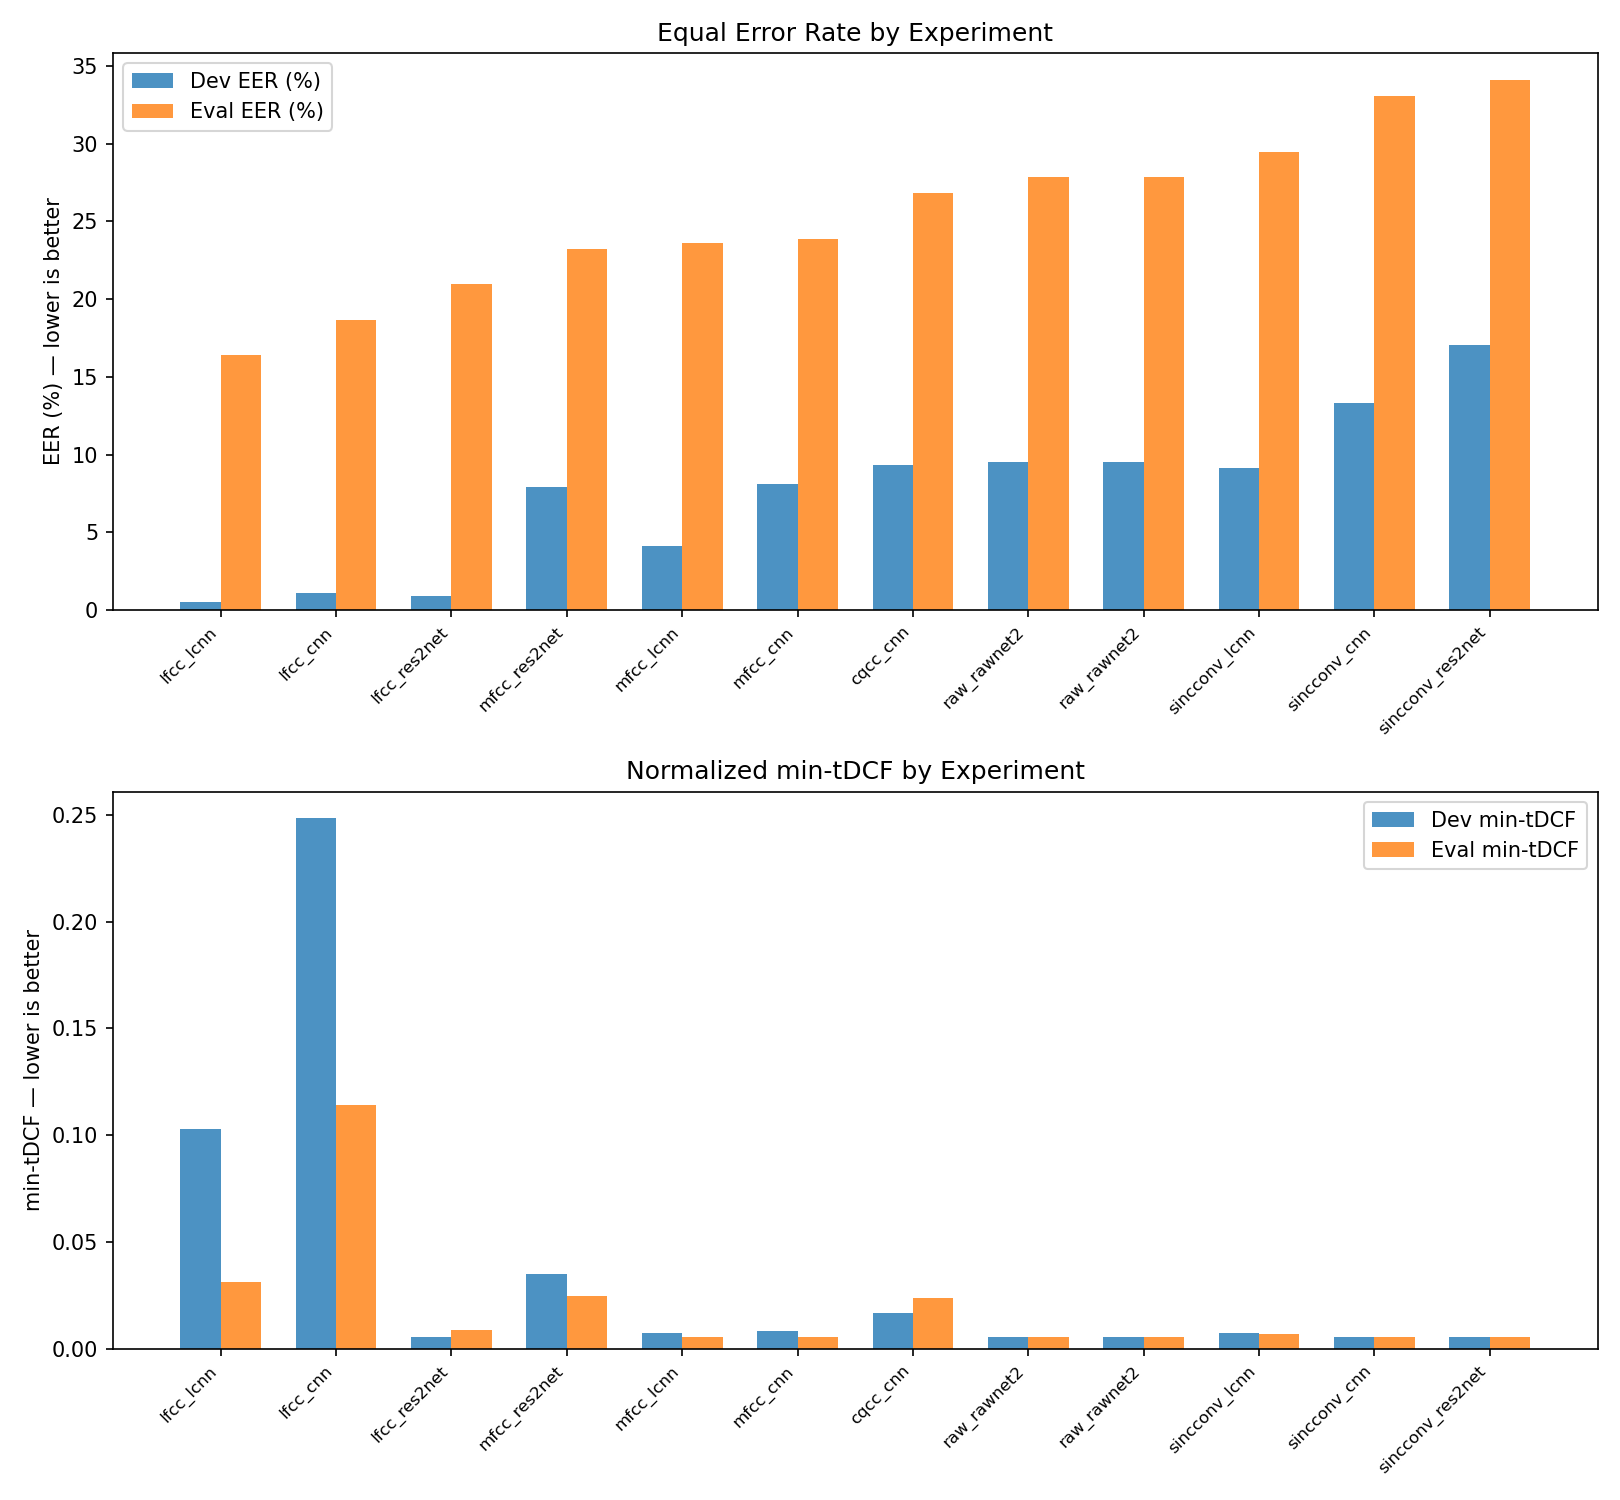
\includegraphics[width=\textwidth]{results_comparison.png}
\caption{Eval EER comparison across experiments --- lower is better}
\label{fig:comparison}
\end{figure}

\section{Training Curves}

Training loss and accuracy curves for each experiment are shown in
Figures~\ref{fig:curves-mfcc}--\ref{fig:curves-raw}.

\begin{figure}[h!]
\centering
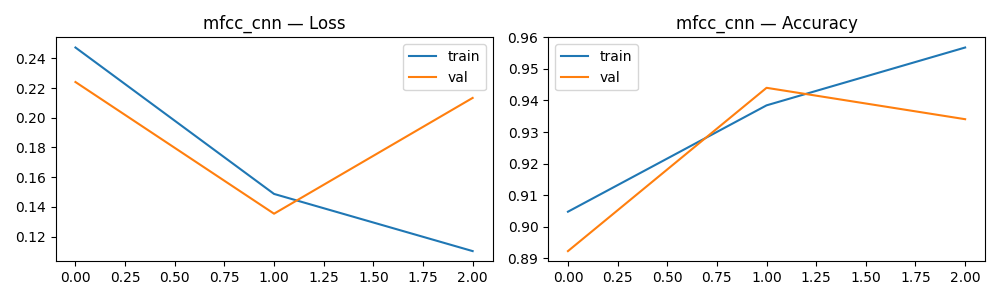
\includegraphics[width=0.48\textwidth]{mfcc_cnn_curve.png}\hfill
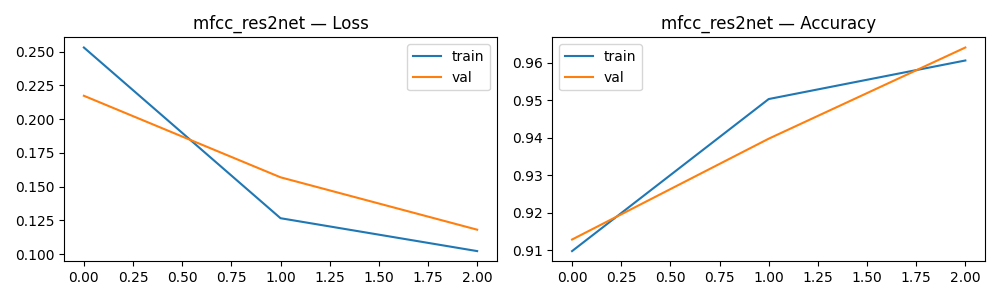
\includegraphics[width=0.48\textwidth]{mfcc_res2net_curve.png}\\[0.5em]
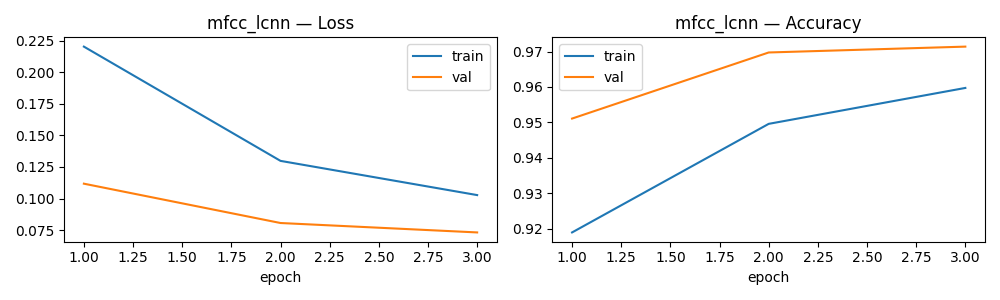
\includegraphics[width=0.48\textwidth]{mfcc_lcnn_curve.png}
\caption{Training curves for MFCC combinations}
\label{fig:curves-mfcc}
\end{figure}

\begin{figure}[h!]
\centering
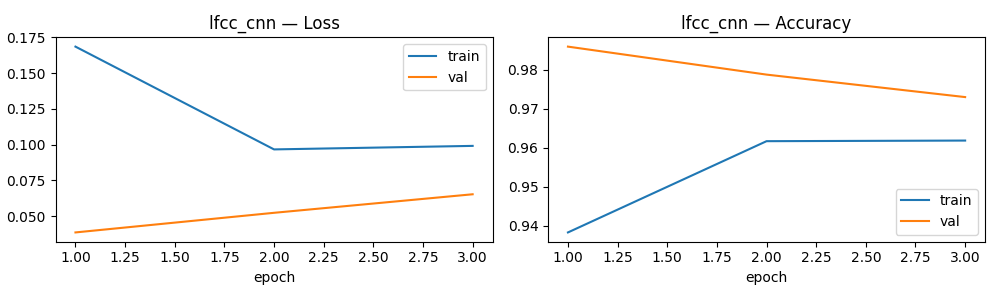
\includegraphics[width=0.48\textwidth]{lfcc_cnn_curve.png}\hfill
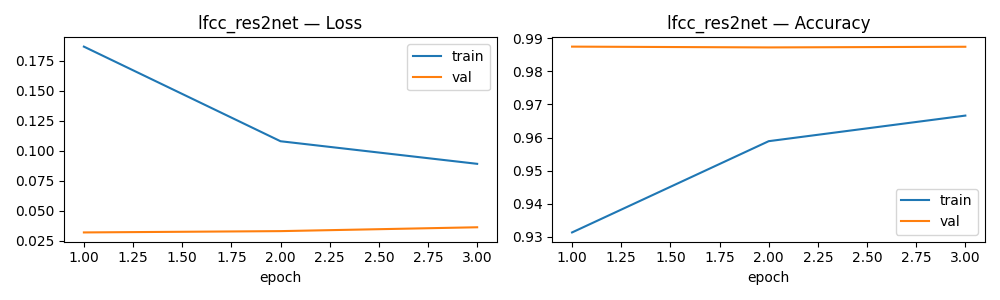
\includegraphics[width=0.48\textwidth]{lfcc_res2net_curve.png}\\[0.5em]
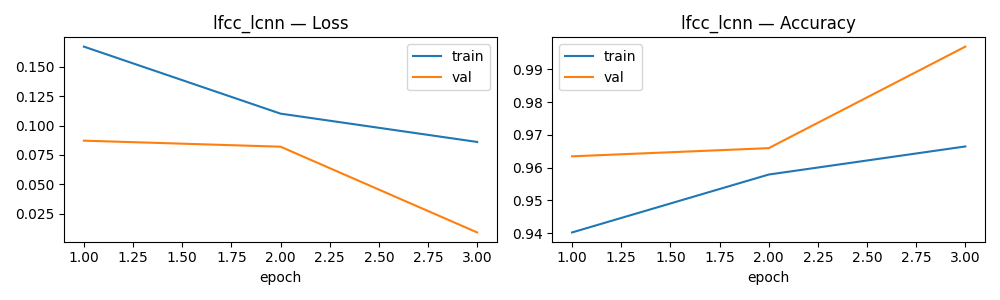
\includegraphics[width=0.48\textwidth]{lfcc_lcnn_curve.png}
\caption{Training curves for LFCC combinations}
\label{fig:curves-lfcc}
\end{figure}

\begin{figure}[h!]
\centering
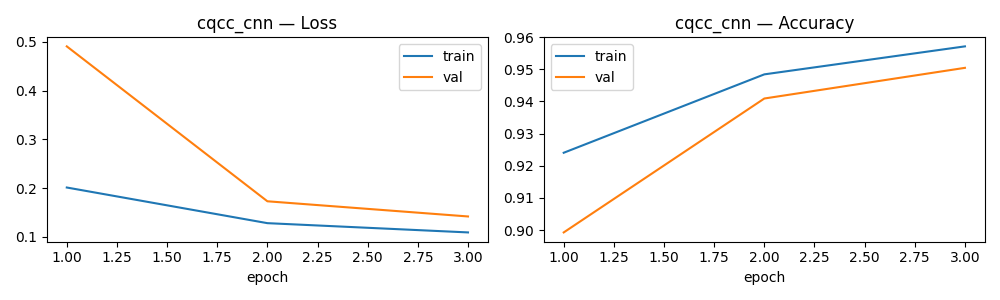
\includegraphics[width=0.48\textwidth]{cqcc_cnn_curve.png}
\caption{Training curve for CQCC+CNN}
\label{fig:curves-cqcc}
\end{figure}

\begin{figure}[h!]
\centering
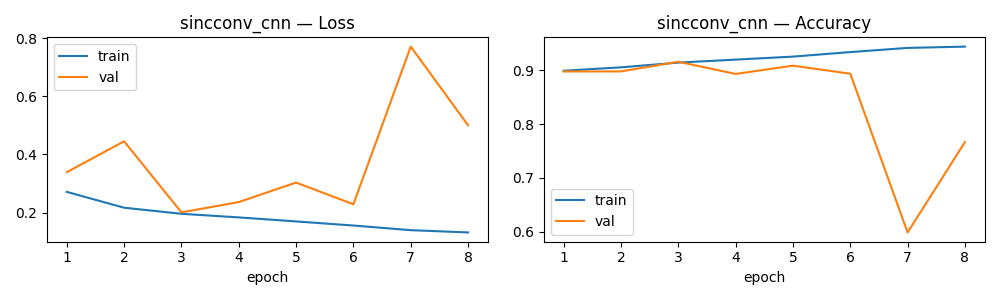
\includegraphics[width=0.48\textwidth]{sincconv_cnn_curve.png}\hfill
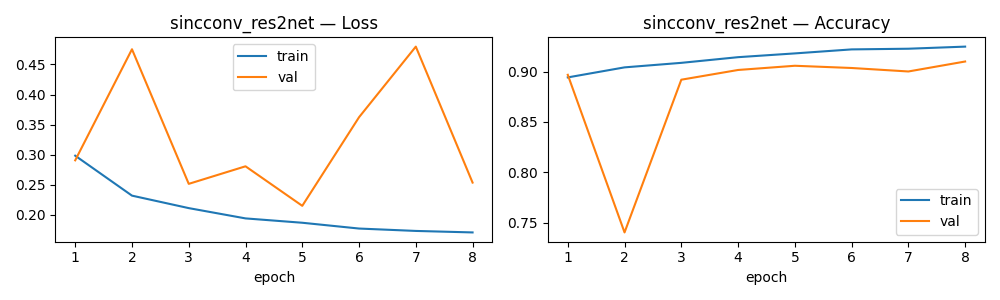
\includegraphics[width=0.48\textwidth]{sincconv_res2net_curve.png}\\[0.5em]
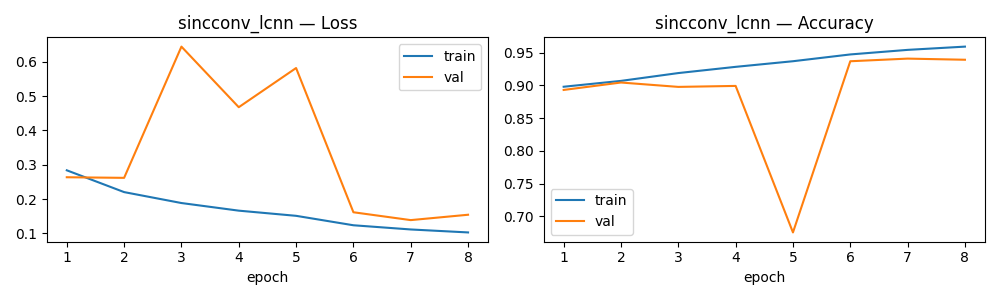
\includegraphics[width=0.48\textwidth]{sincconv_lcnn_curve.png}
\caption{Training curves for SincConv combinations}
\label{fig:curves-sinc}
\end{figure}

\begin{figure}[h!]
\centering
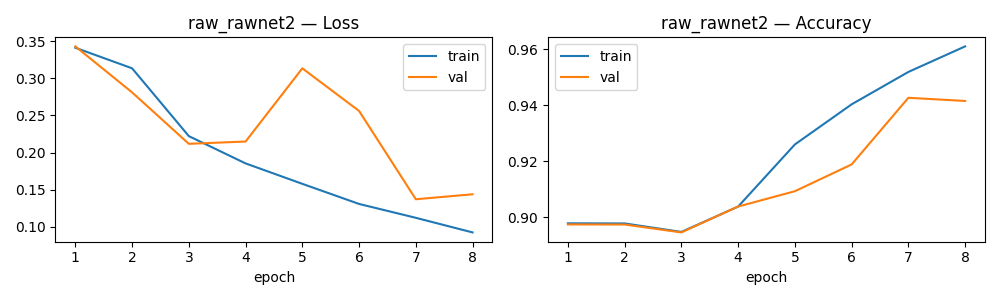
\includegraphics[width=0.48\textwidth]{raw_rawnet2_curve.png}
\caption{Training curve for RawNet2}
\label{fig:curves-raw}
\end{figure}


% =============================================================
\chapter{Discussion and Conclusion}
% =============================================================

\section{Feature Analysis}

\begin{table}[h!]
\centering
\caption{Average Eval EER by feature extractor}
\label{tab:feature-avg}
\begin{tabularx}{0.72\textwidth}{lcc}
\toprule
\textbf{Feature} & \textbf{Mean Eval EER\%} & \textbf{Experiments} \\
\midrule
LFCC     & 18.67 & 3 \\
MFCC     & 23.56 & 3 \\
CQCC     & 26.82 & 1 \\
Raw      & 27.86 & 1 \\
SincConv & 32.22 & 3 \\
\bottomrule
\end{tabularx}
\end{table}

\textbf{LFCC achieves the best average performance} across all feature extractors. The linear
filterbank preserves high-frequency information that is crucial for detecting synthesis artifacts.
As discussed in Section~4.2, vocoders and TTS systems introduce spectral irregularities above
4\,kHz that mel-scaled features (MFCC) attenuate.

\textbf{MFCC ranks second.} Despite its high-frequency attenuation, MFCC still captures
sufficient spectral envelope information for reasonable discrimination, particularly for attack
types that introduce artifacts across the full spectrum.

\textbf{CQCC}, tested only with CNN (the other two combinations failed), performs worse than
both LFCC and MFCC. While CQT's variable resolution is theoretically appealing, the single
successful experiment is insufficient to draw strong conclusions. The resampling step required
for uniform-time DCT may also introduce interpolation artifacts.

\textbf{SincConv performs worst.} The learnable filterbank requires substantial training to
optimize its filter boundaries. With only 8 effective training epochs, the filters likely
did not converge far from their mel-scale initialization, resulting in a suboptimal configuration.
Longer training schedules (50+ epochs) have been shown to yield significantly better results
with SincConv-based models in the literature.

\section{Architecture Analysis}

\begin{table}[h!]
\centering
\caption{Average Eval EER by architecture (shared features only)}
\label{tab:arch-avg}
\begin{tabularx}{0.72\textwidth}{lcc}
\toprule
\textbf{Architecture} & \textbf{Mean Eval EER\%} & \textbf{Notes} \\
\midrule
LCNN    & 23.14 & Best average performance \\
CNN     & 25.19 & Simplest architecture \\
Res2Net & 26.11 & Most complex architecture \\
RawNet2 & 27.86 & End-to-end only \\
\bottomrule
\end{tabularx}
\end{table}

\textbf{LCNN with MFM activation achieves the best average results.} The competitive feature
selection mechanism of MFM (Section~5.3) provides an implicit form of feature selection that
helps the network focus on discriminative spectral patterns. The lightweight nature of LCNN
also means fewer parameters to train, which is advantageous with limited training epochs.

\textbf{Vanilla CNN is surprisingly competitive}, ranking second despite having no attention
mechanisms or residual connections. This suggests that with sufficient depth (four blocks) and
standard regularization (BatchNorm, Dropout), a simple CNN can extract adequate discriminative
features from spectrograms.

\textbf{Res2Net does not improve over CNN.} Despite its multi-scale residual connections and
SE attention, Res2Net's additional complexity does not translate to better performance under
our training conditions. The multi-scale mechanism requires more training to realize its
benefits---with 8 epochs, the hierarchical feature cascades may not have converged.

\textbf{RawNet2} underperforms feature-based models. End-to-end learning from raw waveforms
demands more data and longer training to learn effective representations from scratch, compared
to systems that start from well-designed handcrafted features.

\section{The Generalization Gap}

The most striking observation across all experiments is the \textbf{massive gap between Dev
and Eval EER}. Even the best system (LFCC+LCNN) jumps from 0.50\% Dev EER to 16.39\% Eval
EER---a $33\times$ degradation.

This gap has three primary causes:
\begin{enumerate}
    \item \textbf{Attack mismatch:} Dev and train share the same 6 attack types; the eval set
          introduces 13 entirely new algorithms, many based on more advanced neural synthesis.
    \item \textbf{Insufficient training:} 8 epochs is far below the 30--100 epochs typically
          used in ASVspoof submissions. The networks are undertrained and have not learned
          generalizable spoofing artifacts.
    \item \textbf{Limited augmentation:} Only Gaussian/impulsive noise (RawBoost) is applied.
          More diverse augmentation (SpecAugment, codec simulation, real RIRs) would expose
          the model to greater input variability during training.
\end{enumerate}

\section{Conclusion}

\begin{thmbox}{Overall Findings}{conclusion}
    From 11 successful experiments across 4 feature extractors and 4 architectures, three
    main conclusions emerge:

    \begin{enumerate}[noitemsep]
        \item \textbf{LFCC is the best feature extractor:} Its linear filterbank preserves
              high-frequency information where synthesis artifacts are most prominent, yielding
              consistently lower EER than mel-scaled (MFCC) or log-scaled (CQCC) alternatives.

        \item \textbf{LCNN with MFM is the most effective architecture:} The Max-Feature-Map
              activation provides implicit feature selection that outperforms both standard
              ReLU-based CNNs and more complex Res2Net models under constrained training.

        \item \textbf{Generalization remains the core challenge:} The $30\times$+ gap between
              Dev and Eval EER underscores that detecting \emph{known} attacks is far easier
              than generalizing to \emph{unseen} synthesis methods. Addressing this requires
              longer training, richer augmentation, and potentially architecture-level changes
              (e.g., self-supervised pre-training, graph-based models like AASIST).
    \end{enumerate}
\end{thmbox}

\begin{genbox}{Recommendations for Improvement}
\begin{itemize}[noitemsep]
    \item Increase training epochs to at least 30 with active early stopping.
    \item Apply diverse augmentation: SpecAugment, real Room Impulse Responses, codec simulation.
    \item Explore feature fusion (score-level or embedding-level) to combine complementary
          strengths of different features.
    \item Fix the CQCC dimensional mismatch to enable Res2Net and LCNN experiments.
    \item Investigate self-supervised learning (SSL) front-ends (wav2vec 2.0, WavLM) which
          have shown the best generalization in recent ASVspoof editions.
    \item Consider graph-based architectures (AASIST, RawGAT-ST) that model spectro-temporal
          dependencies beyond what CNNs can capture.
\end{itemize}
\end{genbox}


% =============================================================
\appendix
\chapter{Mathematical Foundations}
% =============================================================

This appendix provides the mathematical background for the signal processing and machine
learning concepts used throughout this report.


\section{The Discrete Fourier Transform (DFT)}

The DFT converts a finite-length discrete-time signal $x[n]$, $n = 0, 1, \ldots, N-1$,
into its frequency-domain representation:

\begin{equation}
    X[k] = \sum_{n=0}^{N-1} x[n] \, e^{-j 2\pi k n / N}, \quad k = 0, 1, \ldots, N-1
    \label{eq:dft}
\end{equation}

The inverse DFT recovers the time-domain signal:
\begin{equation}
    x[n] = \frac{1}{N} \sum_{k=0}^{N-1} X[k] \, e^{j 2\pi k n / N}
    \label{eq:idft}
\end{equation}

Each frequency bin $k$ corresponds to the frequency $f_k = k \cdot f_s / N$ Hz, where
$f_s$ is the sampling rate. The frequency resolution is $\Delta f = f_s / N$.

\subsection{Properties of the DFT}

\begin{itemize}
    \item \textbf{Linearity:} $\text{DFT}\{a \cdot x + b \cdot y\} = a \cdot X + b \cdot Y$
    \item \textbf{Parseval's theorem:} Total energy is preserved:
          $\sum_n |x[n]|^2 = \frac{1}{N} \sum_k |X[k]|^2$
    \item \textbf{Conjugate symmetry:} For real-valued $x[n]$: $X[N-k] = X^*[k]$, so only
          the first $N/2 + 1$ bins carry unique information.
    \item \textbf{Circular convolution theorem:} Multiplication in frequency domain equals
          circular convolution in time domain: $\text{DFT}\{x \circledast y\} = X \cdot Y$.
\end{itemize}

\subsection{The Fast Fourier Transform (FFT)}

The FFT (Cooley \& Tukey, 1965) is an algorithm that computes the DFT in $O(N \log N)$
operations instead of the naive $O(N^2)$. It exploits the symmetry and periodicity of the
complex exponential $W_N^{kn} = e^{-j2\pi kn/N}$ by recursively decomposing the $N$-point
DFT into two $N/2$-point DFTs:

\begin{equation}
    X[k] = \underbrace{\sum_{m=0}^{N/2-1} x[2m] \, W_{N/2}^{mk}}_{\text{DFT of even samples}}
         + W_N^k \underbrace{\sum_{m=0}^{N/2-1} x[2m+1] \, W_{N/2}^{mk}}_{\text{DFT of odd samples}}
\end{equation}

This decomposition is applied recursively until the base case of 2-point DFTs, yielding
$\log_2 N$ levels with $O(N)$ operations each.

For our $N_\text{FFT} = 512$: naive DFT would require $512^2 = 262\,144$ complex multiplications;
FFT requires only $512 \times 9 \approx 4\,608$ --- a $57\times$ speedup.


\section{The Discrete Cosine Transform (DCT)}

The DCT is a real-valued transform closely related to the DFT. The \textbf{Type-II DCT}
(the variant used in MFCC/LFCC/CQCC computation) transforms a sequence $x[n]$ of length $N$:

\begin{equation}
    C[k] = \sum_{n=0}^{N-1} x[n] \cos\!\left[\frac{\pi k (2n + 1)}{2N}\right], \quad k = 0, 1, \ldots, N-1
    \label{eq:dct2}
\end{equation}

With orthonormal normalization (used in our implementation):
\begin{equation}
    C[k] = w_k \sum_{n=0}^{N-1} x[n] \cos\!\left[\frac{\pi k (2n + 1)}{2N}\right],
    \quad w_k = \begin{cases} \sqrt{1/N} & k = 0 \\ \sqrt{2/N} & k > 0 \end{cases}
\end{equation}

\subsection{Why DCT for Cepstral Coefficients?}

The DCT is used in the final stage of MFCC/LFCC/CQCC extraction for three reasons:

\begin{enumerate}
    \item \textbf{Decorrelation:} Mel/linear filterbank outputs are correlated because adjacent
          triangular filters overlap. The DCT is the \textbf{optimal decorrelating transform}
          for signals whose autocorrelation matrix is Toeplitz (a good approximation for
          filterbank energies). Decorrelated features reduce redundancy and improve the
          conditioning of downstream classifiers.

    \item \textbf{Energy compaction:} The DCT concentrates most of the signal energy into the
          first few coefficients. For the log-filterbank spectrum, the low-order DCT
          coefficients capture the broad spectral envelope (vocal tract shape), while
          high-order coefficients capture fine spectral details (pitch harmonics). This
          natural separation allows truncation to $N_\text{MFCC} \ll M$ coefficients with
          minimal information loss.

    \item \textbf{Cepstral domain:} The DCT of the log-spectrum is the \emph{cepstrum}
          (an anagram of ``spectrum''). In the cepstral domain, the convolutive effects
          of the source-filter model (excitation convolved with vocal tract impulse response)
          become \emph{additive}, making them easier to separate. Low-order cepstral
          coefficients represent the filter (vocal tract), while high-order ones represent
          the source (glottal excitation).
\end{enumerate}


\section{The Mel Scale}

The mel scale (Stevens et al., 1937) is a \textbf{perceptual scale of pitch} that maps
physical frequency (Hz) to perceived pitch. It is approximately linear below 1\,kHz and
logarithmic above.

\begin{equation}
    m = 2595 \cdot \log_{10}\!\left(1 + \frac{f}{700}\right)
\end{equation}

\begin{equation}
    f = 700 \cdot \left(10^{m/2595} - 1\right)
\end{equation}

\subsection{Psychoacoustic Basis}

The mel scale approximates the \textbf{critical band} structure of the human cochlea.
The basilar membrane in the inner ear resonates at different positions for different
frequencies, with:
\begin{itemize}[noitemsep]
    \item High spatial resolution (narrow critical bands) at low frequencies --- this is why
          we can distinguish tones 100\,Hz apart below 1\,kHz but cannot distinguish tones
          100\,Hz apart at 8\,kHz.
    \item Progressively wider critical bands at higher frequencies --- the cochlea has
          approximately 24 critical bands (Barks) spanning 20\,Hz to 20\,kHz.
\end{itemize}

A mel-spaced filterbank mirrors this structure: narrow filters at low frequencies (high
resolution where human perception is keen) and wide filters at high frequencies (low
resolution where perception is coarse). This is optimal for speech recognition (matching
human perception) but suboptimal for spoofing detection (where high-frequency artifacts
carry discriminative information).


\section{The Sinc Function and Ideal Filters}

The \textbf{sinc function} arises naturally as the impulse response of an ideal lowpass filter:

\begin{equation}
    \text{sinc}(x) = \frac{\sin(\pi x)}{\pi x}, \quad \text{sinc}(0) = 1
\end{equation}

An ideal lowpass filter with cutoff $f_c$ (normalized to the sampling rate) passes all
frequencies below $f_c$ and blocks all frequencies above. Its impulse response is:

\begin{equation}
    h[n] = 2f_c \cdot \text{sinc}(2f_c n) = \frac{\sin(2\pi f_c n)}{\pi n}
\end{equation}

\subsection{Properties}

\begin{itemize}
    \item The sinc function has \textbf{infinite support}: it extends to $\pm\infty$ and
          decays as $1/n$. In practice, it must be truncated (windowed) to a finite length.
    \item It oscillates with decreasing amplitude, and its zeros occur at integer multiples
          of $1/(2f_c)$.
    \item The frequency response of the truncated (windowed) sinc is no longer an ideal
          rectangle but has \textbf{ripples} (Gibbs phenomenon). The window function controls
          the tradeoff between main-lobe width (transition bandwidth) and side-lobe level
          (stopband attenuation).
\end{itemize}

\subsection{Bandpass Construction}

A bandpass filter passing $[f_1, f_2]$ is constructed as the difference of two lowpass filters:

\begin{equation}
    h_\text{BP}[n] = h_\text{LP}(f_2)[n] - h_\text{LP}(f_1)[n]
                   = 2f_2 \,\text{sinc}(2f_2 n) - 2f_1 \,\text{sinc}(2f_1 n)
\end{equation}

In the frequency domain, this corresponds to $H_\text{BP}(f) = H_\text{LP}(f_2) - H_\text{LP}(f_1)$,
which equals 1 for $f_1 \leq |f| \leq f_2$ and 0 elsewhere.


\section{Window Functions}

Window functions taper the edges of a finite-length signal segment to reduce spectral leakage.

\subsection{Rectangular Window}

The simplest window (equivalent to no windowing):
\begin{equation}
    w[n] = 1, \quad 0 \leq n \leq N-1
\end{equation}
Produces the narrowest main lobe (best frequency resolution) but the highest side lobes
($-13$\,dB), causing severe spectral leakage.

\subsection{Hann Window}

\begin{equation}
    w[n] = 0.5 - 0.5\cos\!\left(\frac{2\pi n}{N-1}\right)
\end{equation}
Reduces side lobes to $-31$\,dB at the cost of a wider main lobe. Commonly used in STFT
computations for speech processing.

\subsection{Hamming Window}

\begin{equation}
    w[n] = 0.54 - 0.46\cos\!\left(\frac{2\pi n}{N-1}\right)
\end{equation}
The Hamming window is a modified Hann window that does \emph{not} reach zero at the endpoints.
This reduces the nearest side lobe to $-43$\,dB (compared to Hann's $-31$\,dB), providing
better stopband attenuation. It is used in our SincConv implementation to window the
truncated sinc kernels.

\subsection{Tradeoff}

All window functions present a fundamental tradeoff between:
\begin{itemize}[noitemsep]
    \item \textbf{Main-lobe width} (frequency resolution): narrower is better for resolving
          closely-spaced frequency components.
    \item \textbf{Side-lobe level} (spectral leakage): lower is better for detecting weak
          components near strong ones.
\end{itemize}
No window can simultaneously optimize both---this is a consequence of the uncertainty principle
for discrete signals.


\section{The Convolution Theorem}

The \textbf{convolution theorem} states that convolution in one domain corresponds to
point-wise multiplication in the other:

\begin{equation}
    x[n] * h[n] \;\xleftrightarrow{\text{DFT}}\; X[k] \cdot H[k]
\end{equation}

\begin{equation}
    x[n] \cdot h[n] \;\xleftrightarrow{\text{DFT}}\; \frac{1}{N} X[k] * H[k]
\end{equation}

This theorem is foundational to:
\begin{itemize}
    \item \textbf{Filterbank design:} Applying a filter in the time domain (convolution with
          its impulse response) is equivalent to multiplying in the frequency domain.
    \item \textbf{STFT interpretation:} The STFT can be viewed as applying a bank of
          frequency-shifted analysis filters to the signal.
    \item \textbf{Source-filter model:} Speech is modeled as the convolution of a glottal
          excitation source with the vocal tract filter. In the log-spectral (cepstral) domain,
          this convolution becomes addition, enabling separation of source and filter
          characteristics.
\end{itemize}

\begin{thmbox}{Source-Filter Separation in the Cepstral Domain}{source-filter}
    If speech $s[n] = e[n] * v[n]$ (excitation $e$ convolved with vocal tract $v$), then:
    \begin{align}
        |S(f)|^2 &= |E(f)|^2 \cdot |V(f)|^2 \\
        \log|S(f)|^2 &= \log|E(f)|^2 + \log|V(f)|^2 \\
        \text{DCT}\{\log|S|^2\} &= \text{DCT}\{\log|E|^2\} + \text{DCT}\{\log|V|^2\}
    \end{align}

    Low-order cepstral coefficients correspond to the slowly-varying vocal tract envelope
    $V(f)$, while high-order coefficients capture the rapidly-varying excitation harmonics
    $E(f)$. This separation is why cepstral features are so effective for speech analysis:
    they naturally disentangle the two fundamental components of speech production.

    For spoofing detection, this is relevant because synthetic speech often has unnatural
    excitation patterns (e.g., perfectly periodic F0, absence of micro-perturbations) that
    manifest in the high-order cepstral coefficients.
\end{thmbox}


\end{document}
